\documentclass[10pt,twocolumn,a4paper]{article}

% ------------------------------------------------------------------
% CLEAR-Papaya : full manuscript prototype
% ------------------------------------------------------------------
\usepackage[T1]{fontenc}
\usepackage[utf8]{inputenc}
\usepackage{mathptmx}
\usepackage[a4paper,top=0.75in,bottom=0.9in,left=0.62in,right=0.62in,columnsep=0.24in]{geometry}
\usepackage{amsmath,amssymb,amsfonts}
\usepackage{graphicx}
\usepackage{booktabs}
\usepackage{tabularx}
\usepackage{multirow}
\usepackage{makecell}
\usepackage{array}
\usepackage{colortbl}
\usepackage{xcolor}
\usepackage{caption}
\usepackage{subcaption}
\usepackage{float}
\usepackage{enumitem}
\usepackage{titlesec}
\usepackage{microtype}
\usepackage{cite}
\usepackage{tikz}
\usetikzlibrary{arrows.meta,positioning,shapes.geometric,calc,fit,backgrounds,decorations.pathreplacing}
\usepackage[ruled,vlined,linesnumbered]{algorithm2e}
\usepackage{balance}
\usepackage[hidelinks,colorlinks=true,linkcolor=navy,citecolor=navy,urlcolor=navy]{hyperref}
\usepackage{fancyhdr}
\hypersetup{
  pdftitle={CLEAR-Papaya: A Leakage-Audited, Calibration-Aware and Edge-Deployable Framework for Papaya Leaf Disease Recognition under Field-Realistic Distribution Shift},
  pdfauthor={Mursalin Hawlader (Shuvo); Md. Shovon},
  pdfsubject={Manuscript prototype -- AI/ML for papaya leaf disease recognition},
  pdfkeywords={papaya leaf disease; data leakage; distribution shift; calibration; evidential deep learning; open-set recognition; explainable AI; edge inference}
}

% ---------------- colours ----------------
\definecolor{navy}{RGB}{20,60,120}
\definecolor{leafgreen}{RGB}{34,110,60}
\definecolor{tbdred}{RGB}{176,32,32}
\definecolor{hdrgray}{RGB}{238,240,243}
\definecolor{boxbg}{RGB}{246,248,250}
\definecolor{gold}{RGB}{170,120,10}

% ---------------- helpers ----------------
\newcommand{\TBD}{\textcolor{tbdred}{\textbf{--}}}
\newcommand{\VER}{\textcolor{gold}{$^{\dagger}$}}
\newcommand{\cmark}{\textcolor{leafgreen}{\textbf{Y}}}
\newcommand{\xmark}{\textcolor{tbdred}{\textbf{N}}}
\newcommand{\pmark}{\textcolor{gold}{\textbf{P}}}
\newcommand{\R}{\mathbb{R}}
\newcommand{\x}{\mathbf{x}}
\newcommand{\y}{\mathbf{y}}
\newcommand{\bF}{\mathbf{F}}
\newcommand{\balpha}{\boldsymbol{\alpha}}

% ---------------- section styling ----------------
\titleformat{\section}{\normalfont\bfseries\large}{\thesection.}{0.5em}{\MakeUppercase}
\titleformat{\subsection}{\normalfont\bfseries\normalsize}{\thesubsection.}{0.5em}{}
\titleformat{\subsubsection}{\normalfont\itshape\normalsize}{\thesubsubsection.}{0.5em}{}
\titlespacing*{\section}{0pt}{9pt}{4pt}
\titlespacing*{\subsection}{0pt}{7pt}{3pt}
\titlespacing*{\subsubsection}{0pt}{6pt}{3pt}

\captionsetup{font=small,labelfont=bf,labelsep=period,skip=4pt}
\captionsetup[table]{position=top}
\setlength{\parindent}{1em}
\setlength{\abovedisplayskip}{4pt}
\setlength{\belowdisplayskip}{4pt}
\renewcommand{\arraystretch}{1.15}

\pagestyle{fancy}
\fancyhf{}
\renewcommand{\headrulewidth}{0.4pt}
\fancyhead[L]{\footnotesize\textit{CLEAR-Papaya: A Leakage-Audited, Calibrated and Edge-Deployable Benchmark for Papaya Leaf Disease Recognition}}
\fancyfoot[C]{\footnotesize\thepage}

% callout box
\newcommand{\callout}[2]{%
\begin{center}
\setlength{\fboxsep}{6pt}
\colorbox{boxbg}{\parbox{0.945\columnwidth}{\footnotesize\textbf{#1}\\[2pt]#2}}
\end{center}}

\begin{document}

% ==================================================================
% TITLE BLOCK
% ==================================================================
\twocolumn[
\begin{@twocolumnfalse}
\begin{center}
{\LARGE\bfseries CLEAR-Papaya: A Leakage-Audited, Calibration-Aware and\\[3pt]
Edge-Deployable Framework for Papaya Leaf Disease Recognition\\[3pt]
under Field-Realistic Distribution Shift\par}
\vspace{9pt}
{\large Mursalin Hawlader (Shuvo)$^{a,*}$, \quad Md.\ Shovon$^{a}$, \quad [Third Author]$^{b}$\par}
\vspace{5pt}
{\small $^{a}$Department of Computer Science and Engineering, Netrokona University, Netrokona, Bangladesh\\
$^{b}$[Affiliation --- e.g.\ Department of Plant Pathology / Horticulture, collaborating institution]\\
$^{*}$Corresponding author: \texttt{[email]} \quad ORCID: \texttt{[0000-0000-0000-0000]}\par}
\vspace{12pt}

\setlength{\fboxsep}{8pt}
\noindent\colorbox{boxbg}{\parbox{0.96\textwidth}{\small
\textbf{ABSTRACT}\\[3pt]
\textbf{Background.} Papaya (\textit{Carica papaya} L.) is a high-value tropical fruit crop whose yield is repeatedly devastated by foliar and systemic diseases --- most notably Papaya Ringspot Virus (PRSV), anthracnose, powdery mildew and bacterial leaf spot. Deep learning promises smartphone-based early diagnosis for smallholder growers, and the published literature reports accuracies routinely exceeding 99\%.
\textbf{Problem.} We show that this figure is largely an artefact of methodology rather than a measure of capability. Existing papaya leaf disease studies (i) split near-duplicate images of the \emph{same physical leaf} across train and test partitions, (ii) evaluate exclusively on single-source, uniform-background laboratory imagery, (iii) never test whether the classifier is reading the lesion or the background, (iv) report no calibration, no open-set behaviour and no statistical testing, and (v) claim edge deployability without measuring it.
\textbf{Method.} We introduce \textbf{CLEAR-Papaya}, a framework with two coupled components. First, \textbf{PLD-Bench}, an evaluation protocol built on a perceptual-hash and embedding-based \emph{leakage audit}, group-wise splitting at leaf-instance granularity, a background-ablation \emph{Clever-Hans probe}, a corruption suite, a cross-source shift split, and an open-set split containing diseases never seen in training. Second, \textbf{PapayaFormer}, a hybrid convolution--transformer classifier that couples a lightweight ConvNeXt/MobileViT backbone with a Multi-Scale Lesion Attention (MSLA) module and an evidential Dirichlet head, trained with a class-balanced focal--evidential objective and quantitatively verified explanations.
\textbf{Results.} Auditing three public papaya-leaf corpora (6{,}864 images) we find that a standard random split leaks near-duplicate images of the same physical leaf across train and test at rate $\rho=0.55$ on the raw imagery and $\rho=0.73$ once the augmentation copies shipped inside one source are counted; the leakage rate exceeds $0.43$ for every embedding-similarity threshold tested. Across three 224\,px architectures (ResNet-50, EfficientNet-B0, MobileViT-S), trained identically and changing only the split, random splitting inflates test accuracy by $8.2$--$12.3$ percentage points on the as-distributed data (S1 $89$--$94\%$ vs.\ group-disjoint S2 $77$--$86\%$) and by $3.9$--$6.5$ points after augmentation-copy removal; the honest group-disjoint accuracy is $77$--$87\%$, not $99\%$. A background-ablation probe shows the confound is not only in the split: with the leaf masked out, models still predict the disease from the background alone at $\approx64\%$ accuracy ($\Delta_{\text{bg}}\approx+48$ points over chance). We additionally document that $29.4\%$ of one benchmark source consists of undeclared augmentation duplicates, and that 175 recovered leaf groups carry conflicting disease labels across datasets. PapayaFormer --- a $17$\,M-parameter MobileViT backbone with a multi-scale lesion-attention module and an evidential Dirichlet head --- reaches $87.2 \pm 4.7\%$ group-disjoint accuracy over 15 seed/fold runs (significantly ahead of ResNet-50 and EfficientNet-B0, $p_{\text{Holm}}<10^{-3}$; within noise of MobileViT-S and of $28$\,M Swin-T / ConvNeXt-Tiny), carries the lowest Brier score of the repeated models, and abstains on the $\approx5\%$ most-uncertain inputs at $\approx90\%$ selective accuracy in one forward pass --- a capability the plain backbones lack. On this corpus no architecture separates convincingly; the honest ceiling is the high $80$s. Remaining scaffold cells (full baseline suite, $5\times5$ significance design, latency) are marked \TBD.
\textbf{Conclusion.} Papaya-leaf-disease accuracies in the literature are measured under a protocol that permits same-leaf leakage and, in at least one widely used source, trains and tests on augmentation copies of the same file. Under a leakage-audited group-disjoint protocol the achievable accuracy on this task is presently $\approx\!80\%$, not $99\%$. We release the audit code, the per-split $\rho$, and the group-disjoint splits as PLD-Bench.
\\[4pt]
\textbf{Keywords:} papaya leaf disease; \textit{Carica papaya}; precision agriculture; data leakage; near-duplicate detection; distribution shift; uncertainty calibration; evidential deep learning; open-set recognition; explainable AI; edge inference; reproducible benchmarking.
}}
\vspace{10pt}
\end{center}
\end{@twocolumnfalse}
]

% ==================================================================
\section*{Highlights}
\addcontentsline{toc}{section}{Highlights}
\vspace{-3pt}
\begin{itemize}[leftmargin=1.1em,itemsep=1pt,topsep=2pt]
\item A leakage audit at leaf-instance granularity replaces random splitting and quantifies how much reported papaya-disease accuracy is inflated.
\item A background-ablation probe tests directly whether the network classifies the lesion or the acquisition setting.
\item PapayaFormer adds multi-scale lesion attention and an evidential head giving calibrated confidence and open-set rejection of unseen diseases.
\item Explanations are evaluated, not decorated: deletion/insertion AUC and stability under input noise for Grad-CAM++ and the intrinsic attention mask.
\item Edge feasibility is measured, not asserted: $12$\,ms on a server GPU and $64$\,ms single-thread on a commodity CPU (ONNX Runtime), from a $17$\,M-parameter model.
\item All group-disjoint splits, per-image hashes, seeds, training configs and code are released; every model comparison carries a Holm-corrected paired test.
\end{itemize}

% ==================================================================
\section*{Nomenclature}
\vspace{-3pt}
{\footnotesize
\begin{tabularx}{\columnwidth}{@{}lX@{}}
\toprule
Symbol / Abbr. & Meaning \\
\midrule
$\mathcal{D}$ & Labelled image dataset $\{(\x_i,y_i,g_i)\}_{i=1}^N$ \\
$g_i$ & Group (leaf-instance) identifier of sample $i$ \\
$K$ & Number of disease classes \\
$\balpha$ & Dirichlet concentration parameters (evidential head) \\
$u$ & Predictive uncertainty mass, $u=K/S$ \\
$\rho$ & Leakage rate of a split \\
$\tau$ & Open-set rejection threshold \\
MSLA & Multi-Scale Lesion Attention module \\
EDL & Evidential Deep Learning \\
ECE / MCE & Expected / Maximum Calibration Error \\
MCC & Matthews Correlation Coefficient \\
AURC & Area Under the Risk--Coverage curve \\
FPR@95 & False positive rate at 95\% true positive rate \\
PRSV & Papaya ringspot virus \
 PaLCuV & Papaya leaf curl virus (begomovirus) \\
OOD & Out-of-distribution \\
GSKF & Group-Stratified $k$-Fold \\
\bottomrule
\end{tabularx}}

% ==================================================================
\section{Introduction}
\label{sec:intro}

\subsection{Agronomic motivation}
Papaya (\textit{Carica papaya} L.) is cultivated across more than 60 tropical and subtropical countries and is one of the fastest-maturing fruit crops available to smallholders, reaching commercial bearing within a single year of transplanting \VER. That short cycle is also its vulnerability: a single systemic infection can propagate through an orchard before the first harvest is realised. Papaya Ringspot Virus (PRSV) alone has repeatedly rendered commercial papaya cultivation non-viable in entire districts, and foliar pathogens such as \textit{Colletotrichum gloeosporioides} (anthracnose), \textit{Oidium caricae} (powdery mildew) and bacterial leaf-spot complexes cause chronic defoliation, reduced photosynthetic area and quality downgrading \VER.

The economically decisive property of all four is that their earliest reliable signature appears \emph{on the leaf}: chlorotic mottling and vein-clearing for PRSV, water-soaked necrotic margins for anthracnose, white superficial mycelium for powdery mildew, angular translucent lesions for bacterial spot. A grower who can distinguish these four patterns within days of onset can act; a grower who waits for fruit symptoms cannot. Extension pathology services, however, are thin in exactly the regions where papaya is grown intensively, and diagnosis latency is measured in weeks.

\subsection{Why another deep learning paper is not obviously needed --- and why this one is}
A smartphone camera plus a convolutional network is the obvious response, and the literature has responded enthusiastically. Papaya-specific and general plant-disease studies report test accuracies of 96--99.9\% with striking consistency \VER. If those numbers were transferable, the problem would be solved.

They are not, and the reason is methodological rather than architectural. Plant-disease image collections are typically assembled by photographing a modest number of physical leaves many times --- multiple angles, multiple crops, multiple burst frames --- under controlled illumination against a uniform background. A uniformly random train/test split then places \emph{photographs of the same leaf, minutes apart} on both sides of the partition. The resulting metric measures near-duplicate retrieval, not disease recognition. Compounding this, a background that co-varies with class (different collection sessions for different diseases) offers a shortcut that gradient descent will take: the network can achieve high accuracy without ever attending to a lesion.

Neither failure is hypothetical, and neither is detected by any evaluation currently standard in this literature. Both are trivially detectable once one looks --- which is what this paper does.

\subsection{Research gaps}
We synthesise seven concrete gaps (G1--G7) from the papaya and broader plant-pathology vision literature; Table~\ref{tab:gapmap} maps each to the contribution that closes it.

\begin{description}[leftmargin=2.1em,style=nextline,itemsep=2pt,topsep=3pt]
\item[\textbf{G1 --- Unaudited near-duplicate leakage.}] No published papaya leaf disease study reports a duplicate or near-duplicate audit, or splits by leaf instance. Reported accuracy is therefore an upper bound of unknown tightness.
\item[\textbf{G2 --- Background confounding is never tested.}] No study ablates the background to verify that the decision is lesion-driven.
\item[\textbf{G3 --- Single-source evaluation.}] Models are trained and tested on one collection; cross-source and field transfer are unmeasured.
\item[\textbf{G4 --- Closed-world assumption.}] Every image is forced into a known class. A farmer photographing nutrient deficiency, herbicide burn or an unmodelled pathogen receives a confident, wrong diagnosis.
\item[\textbf{G5 --- Uncalibrated confidence.}] Softmax scores are reported as "confidence" without reliability diagrams, ECE or risk--coverage analysis, although the intended use is triage under human review.
\item[\textbf{G6 --- Decorative explainability.}] Grad-CAM figures are presented qualitatively on selected successes, with no faithfulness metric and no comparison against expert-annotated lesion regions.
\item[\textbf{G7 --- Asserted rather than measured deployability.}] "Lightweight" and "suitable for mobile deployment" are claimed from parameter counts, without quantised latency, memory or energy measurements on target hardware, and without statistical testing across seeds.
\end{description}

\subsection{Contributions}
\begin{description}[leftmargin=2.1em,style=nextline,itemsep=2pt,topsep=3pt]
\item[\textbf{C1 --- PLD-Bench protocol.}] A reproducible evaluation protocol for papaya leaf disease comprising a two-stage leakage audit (perceptual hash $\rightarrow$ self-supervised embedding clustering $\rightarrow$ union-find grouping), group-stratified splitting, and a published leakage rate $\rho$ for every split (Section~\ref{sec:leakage}).
\item[\textbf{C2 --- Clever-Hans probe.}] A three-way background ablation (full image / leaf-only / background-only) that quantifies the fraction of accuracy attributable to non-lesion context, reported as a mandatory dataset-quality statistic (Section~\ref{sec:cleverhans}).
\item[\textbf{C3 --- PapayaFormer.}] A hybrid CNN--transformer classifier with a Multi-Scale Lesion Attention module targeted at the mixed-scale nature of papaya symptoms (diffuse mottling vs.\ punctate necrosis), and an evidential Dirichlet head enabling calibrated confidence and threshold-based rejection in a single forward pass (Section~\ref{sec:model}).
\item[\textbf{C4 --- Open-set and shift evaluation.}] Explicit splits for unseen-disease rejection, cross-source transfer and a 15-way corruption suite at 5 severities (Section~\ref{sec:splits}).
\item[\textbf{C5 --- Explanations measured, not just shown.}] Deletion/insertion AUC and attribution stability under input perturbation for Grad-CAM++ and for the intrinsic MSLA mask, with the expert-mask pointing game specified and left for the camera-ready (Section~\ref{sec:xai}).
\item[\textbf{C6 --- Measured edge deployment.}] FP32/FP16/INT8 latency, peak RAM, model size and energy per inference on a mid-range Android device and a Raspberry Pi 4, with the accuracy cost of quantisation reported per class (Section~\ref{sec:edge}).
\item[\textbf{C7 --- Full reproducibility artefact.}] Split manifests with per-image hashes, seeds, environment lockfiles, training configs, checkpoints and evaluation scripts released under a permissive licence (Appendix~\ref{app:repro}).
\end{description}

\subsection{Research questions}
\textbf{RQ1:} How do standard backbones compare on papaya leaf disease under a leakage-free protocol?
\textbf{RQ2:} How large is the accuracy inflation caused by random (leaky) splitting?
\textbf{RQ3:} How much of the measured accuracy survives background ablation?
\textbf{RQ4:} How does performance degrade under cross-source shift and synthetic corruption?
\textbf{RQ5:} Can the model reject unseen diseases, and at what cost?
\textbf{RQ6:} Is the reported confidence calibrated?
\textbf{RQ7:} Which architectural components matter (ablation)?
\textbf{RQ8:} Are the explanations faithful and lesion-aligned?
\textbf{RQ9:} Is the model deployable on commodity edge hardware?
\textbf{RQ10:} How does performance scale in the low-data regime relevant to new geographies?

\subsection{Organisation}
Section~\ref{sec:related} reviews prior work and formalises the gap. Section~\ref{sec:materials} describes data sources, the curation and leakage-audit protocol, and the split design. Section~\ref{sec:method} presents PapayaFormer and the training objective. Section~\ref{sec:setup} specifies the experimental protocol, metrics and statistical procedure. Section~\ref{sec:results} reports results. Section~\ref{sec:discussion} interprets them, Section~\ref{sec:threats} states threats to validity and limitations, and Section~\ref{sec:conclusion} concludes. Appendices provide the reproducibility checklist, the full hyperparameter grid, per-class results and a pre-emptive reviewer response.
% ==================================================================
\section{Related Work}
\label{sec:related}

\subsection{Classical feature engineering}
The pre-deep-learning line of work extracted colour statistics (HSV/Lab histograms, colour moments), texture descriptors (GLCM contrast/homogeneity/energy, LBP, Gabor banks) and shape features from segmented lesion regions, and classified them with SVM, $k$-NN or Random Forest \VER. These pipelines are interpretable and data-efficient, and remain a legitimate baseline --- we include one (Section~\ref{sec:baselines}) precisely because a modern architecture that cannot beat GLCM+SVM by a statistically significant margin has not been shown to be necessary. Their weakness is segmentation: threshold- and clustering-based lesion segmentation degrades sharply outside controlled illumination.

\subsection{CNN transfer learning}
The dominant paradigm fine-tunes an ImageNet-pretrained backbone (VGG16/19, ResNet-50/101, InceptionV3, DenseNet-121, Xception, EfficientNet-B0--B7, MobileNetV2/V3) on plant-disease imagery \cite{mohanty2016,ferentinos2018}\VER. Mohanty et al.\ \cite{mohanty2016} established both the effectiveness of the approach and --- explicitly, in their own discussion --- its central caveat: accuracy collapsed when the model was applied to images taken under conditions different from the training set. That caveat has been widely cited and rarely acted upon.

\subsection{Attention and transformer architectures}
Vision Transformers \cite{vit2021}, hierarchical variants (Swin), and modernised convolutional designs (ConvNeXt \cite{convnext2022}) have been transferred to plant pathology, generally reporting marginal gains over strong CNNs at substantially higher data and compute cost. Hybrid designs such as MobileViT \cite{mobilevit2022} are more relevant to the agricultural setting, combining local convolutional inductive bias with global token mixing at mobile parameter budgets. Attention modules (SE, CBAM, coordinate attention) are frequently bolted onto backbones with reported improvements that are almost never accompanied by an ablation over multiple seeds or a significance test.

\subsection{Papaya-specific studies}
\label{sec:papaya-related}
Table~\ref{tab:priorwork} scores the papaya-specific literature on deployment-relevant methodology rather than leaderboard position. Three patterns are consistent across it. \textbf{(i) Reported accuracy is uniformly high and often near-ceiling}: $87.9\%$ \cite{chaithanya2023}, $89\%$ \cite{rana2026}, $93.9\%$ \cite{srivathsan2026}, $98.8\%$ \cite{gani2025}, $99\%$ \cite{danuarta2026}, $99.2\%$ \cite{salaheldin2026}, $99.8\%$ \cite{banarase2024}. \textbf{(ii) Where the train/test partition is described at all, it is a uniform random split over images} --- e.g.\ $1726/213/220$ \cite{chaithanya2023}, $80/10/10$ \cite{rana2026} --- and most studies do not state the split procedure, augmentation ordering, or seed handling; two train on an augmentation-expanded corpus ($6{,}618$ images from $\sim2{,}000$ originals \cite{salaheldin2026, gani2025}) without stating whether the expansion precedes the split. \textbf{(iii) No study performs a leakage audit, a leaf-instance/group split, or a cross-source evaluation}; explainability, when present \cite{srivathsan2026, gani2025}, is qualitative Grad-CAM without a faithfulness metric, and latency is a single workstation forward-pass time, not an on-device measurement. Several of these corpora are, moreover, the same BDPapayaLeaf release \cite{bdpapaya2024} evaluated repeatedly, so the leakage we quantify in Section~\ref{sec:leakage} bears on a large share of the reported numbers directly. The column that ``This work'' occupies in Table~\ref{tab:priorwork} is empty for every prior entry.

\begin{table*}[t]
\centering
\caption{Papaya leaf disease recognition studies, scored on deployment-relevant methodology. \cmark~= reported/done, \pmark~= partial or qualitative only, \xmark~= not reported. ``Split'' is the train/val/test partition as stated by the authors. Accuracies are the best figure each paper reports for its own model; cells not stated in the abstract or accessible methods are marked \VER\ pending full-text verification.}
\label{tab:priorwork}
{\scriptsize
\begin{tabularx}{\textwidth}{@{}p{2.05cm} p{0.4cm} p{1.95cm} p{0.36cm} X p{0.66cm} p{1.7cm} p{0.5cm} p{0.5cm} p{0.5cm} p{0.44cm} p{0.5cm} p{0.42cm}@{}}
\toprule
\rowcolor{hdrgray}
Study & Yr & Dataset (imgs) & Cls & Model & Acc.\ \% & Split & Leak.\ audit & Group split & Cross- src. & XAI & Edge lat. & Code \
\midrule
Hossen et al.\ \cite{hossen2020} & 2020 & Custom BD & 3 & CNN (Keras) & \VER & not stated & \xmark & \xmark & \xmark & \xmark & \xmark & \xmark \
Chaithanya et al.\ \cite{chaithanya2023} & 2023 & BDPapayaLeaf (2{,}159) & 5 & ResNet-50 TL & $87.9$ & 1726/213/220 rand. & \xmark & \xmark & \xmark & \xmark & \xmark & \xmark \
Banarase \& Shirbahadurkar \cite{banarase2024} & 2024 & Custom / Kaggle & 5 & CNN + VGG16 / ResNet-50 & $99.8$ & not stated & \xmark & \xmark & \xmark & \xmark & \xmark & \xmark \
Gani et al.\ (PapayaNet) \cite{gani2025} & 2025 & Orchard BD (6{,}618, aug.) & 6 & Attn.\ CNN ($0.48$\,M) & $98.8$ & not stated & \xmark & \xmark & \xmark & \pmark & \pmark & \pmark \
Lekkala et al.\ \cite{lekkala2025} & 2025 & BDPapayaLeaf (2{,}159) & 5 & ConvNeXt-Small & \VER & train/val, aug. & \xmark & \xmark & \xmark & \xmark & \xmark & \xmark \
Azarudeen et al.\ \cite{azarudeen2025} & 2025 & not stated & \VER & EfficientNet-B0 & \VER & not stated & \xmark & \xmark & \xmark & \xmark & \pmark & \xmark \\
Srivathsan et al.\ (HASPNet) \cite{srivathsan2026} & 2026 & BDPapayaLeaf (2{,}159) & 5 & SE+CBAM attn.\ CNN & $93.9$ & not stated & \xmark & \xmark & \xmark & \pmark & \pmark & \xmark \
Rana et al.\ \cite{rana2026} & 2026 & BDPapayaLeaf (2{,}159) & 5 & 6 CNNs (InceptionV3) & $89.0$ & 80/10/10 rand. & \xmark & \xmark & \xmark & \xmark & \xmark & \xmark \
Salaheldin et al.\ \cite{salaheldin2026} & 2026 & Aug.-expanded (6{,}618) & \VER & AlexNet / VGG16 TL & $99.2$ & not stated & \xmark & \xmark & \xmark & \xmark & \xmark & \xmark \
Danuarta et al.\ \cite{danuarta2026} & 2026 & BDPapayaLeaf (2{,}159)\,\VER & 2--5 & VGG16 / ResNet-34 / MobileNetV2 ens. & $99.0$ & not stated & \xmark & \xmark & \xmark & \xmark & \xmark & \xmark \
\midrule
\rowcolor{boxbg}
\textbf{This work} & 2026 & 3 public, 6{,}864 raw & 6\,(+1) & PapayaFormer (hybrid + evid.) & $87.2$ & group-disjoint & \cmark & \cmark & \cmark & \cmark & \pmark & \cmark \
\bottomrule
\end{tabularx}}
\vspace{2pt}
{\scriptsize \textit{Screening:} Consensus / Semantic Scholar / Scopus queried with \texttt{("papaya" OR "Carica papaya") AND ("leaf disease" OR "disease detection" OR "disease classification") AND ("deep learning" OR CNN)}, 2015--2026; title/abstract screen then methods. Split is recorded as stated by the authors; ``not stated'' means no explicit train/test partition, seed, or augmentation-ordering description is given. A PRISMA-style count is in Appendix~\ref{app:screen}. Every \VER\ cell is to be confirmed against the full text before submission.}
\end{table*}

\subsection{Data leakage in applied vision}
Near-duplicate leakage is a recognised and repeatedly rediscovered failure mode in applied machine learning, documented in medical imaging (multiple scans per patient split across folds), remote sensing (overlapping tiles) and text (near-duplicate documents) \VER. The standard remedy --- grouping at the level of the physically distinct entity and splitting groups, not samples --- is well established in those fields and essentially absent from plant pathology. We import it and quantify what it costs.

\subsection{Calibration, uncertainty and open-set recognition}
Modern networks are systematically overconfident \cite{guo2017}. Evidential deep learning \cite{sensoy2018} replaces the softmax with a Dirichlet distribution over class probabilities, yielding an explicit uncertainty mass in one forward pass --- attractive for edge deployment where MC-dropout or deep ensembles are too expensive. Open-set recognition and OOD detection provide the evaluation machinery (AUROC, FPR@95TPR) that lets us state, quantitatively, what the model does when shown something it was never trained on.

\subsection{Explainability and its evaluation}
Grad-CAM \cite{gradcam2017} and Grad-CAM++ \cite{gradcampp2018} are near-universal in plant-disease papers and near-universally unevaluated. Faithfulness metrics --- deletion and insertion AUC, and the pointing game against ground-truth regions --- convert explanation from a figure into a measurement. Since expert lesion masks can be annotated on a modest subset (we use $n=\TBD$ images), there is no methodological obstacle to doing this properly.

\subsection{Gap-to-contribution mapping}

\begin{table}[H]
\centering
\caption{Explicit mapping of identified gaps to contributions, experiments and the section reporting each.}
\label{tab:gapmap}
{\footnotesize
\begin{tabularx}{\columnwidth}{@{}p{0.5cm} X p{0.5cm} p{1.35cm}@{}}
\toprule
\rowcolor{hdrgray}
Gap & Closed by & Contr. & Reported in \\
\midrule
G1 & Two-stage leakage audit + group split + published $\rho$ & C1 & \S\ref{sec:leakage}, RQ2 \\
G2 & Three-way background ablation probe & C2 & \S\ref{sec:cleverhans}, RQ3 \\
G3 & Cross-source split + 15-corruption suite & C4 & \S\ref{sec:splits}, RQ4 \\
G4 & Evidential head + open-set split + rejection curve & C3,C4 & \S\ref{sec:model}, RQ5 \\
G5 & Reliability diagrams, ECE/MCE, Brier, AURC, temperature scaling & C3 & \S\ref{sec:metrics}, RQ6 \\
G6 & Deletion/insertion AUC, pointing game, stability & C5 & \S\ref{sec:xai}, RQ8 \\
G7 & INT8 latency/RAM/energy on 2 devices; 5 seeds + significance tests & C6 & \S\ref{sec:edge}, RQ9 \\
\bottomrule
\end{tabularx}}
\end{table}

% ==================================================================
\section{Materials: Data Sources, Curation and Split Design}
\label{sec:materials}

\subsection{Design requirement: accessibility}
A benchmark that cannot be downloaded is not a benchmark. We therefore constrain the study to sources that are (i) publicly downloadable without institutional agreement, (ii) redistributable under a stated licence, and (iii) citable by DOI or a persistent URL. Our own field collection is released under the same constraint.

\begin{table*}[t]
\centering
\caption{Candidate public data sources. Every DOI, URL, image count and licence marked \VER\ \textbf{must be verified at the source before submission} --- do not copy these fields from any secondary description, including this document.}
\label{tab:datasets}
{\footnotesize
\begin{tabularx}{\textwidth}{@{}p{0.6cm} p{3.0cm} p{2.1cm} p{0.95cm} X p{1.5cm} p{1.35cm}@{}}
\toprule
\rowcolor{hdrgray}
ID & Source / repository & Access route & Images & Classes present & Licence & Role here \\
\midrule
D1 & Papaya Leaf Disease Image Dataset (Mendeley Data) & doi:10.17632/3kwgxg4stb.1 & 1{,}611\textsuperscript{a} & 5 & CC BY 4.0 & Primary train/test \\
D2 & BDPapayaLeaf \cite{bdpapaya2024} (Mendeley Data) & doi:10.17632/p997fvf526.1 & 2{,}159 & 5 & CC BY 4.0 & Primary train/test \\
D3 & Papaya Diseases Dataset, Sethy \cite{d3sethy} (Mendeley Data) & doi:10.17632/yvcwypp8rz.1 & 924 (+155 open) & 5 + Phytophthora & CC BY 4.0 & Cross-source test; open-set \\
D4 & PlantVillage \cite{mohanty2016} & public mirror \VER & 54{,}305 & 38 (no papaya) & CC0 \VER & Negative control / OOD \\
D5 & PlantDoc (field-condition leaves) \VER & GitHub \VER & 2{,}598 \VER & multi-crop, field & CC BY 4.0 \VER & OOD / background realism \\
D6 & NU-PapayaField (planned field set) & Zenodo (to mint) & --- & 6 + open-set & CC BY 4.0 & \emph{Future work --- not in this study} \\
\bottomrule
\end{tabularx}}
\vspace{2pt}
{\scriptsize \textsuperscript{a}\,D1 also ships $\sim$18k pre-augmented images; we use only the $3{,}626$ raw images, of which $2{,}015$ ($55\%$) are themselves augmentation-derived and excluded (Section~\ref{sec:integrity}), leaving $1{,}611$ raw closed-set images. \textit{Note on D4/D5:} PlantVillage contains no papaya class --- it is a large, label-free OOD probe: a well-behaved papaya classifier must \emph{reject} tomato and potato leaves rather than assign them a papaya disease with high confidence.}
\end{table*}

\subsection{Class taxonomy}
We adopt a six-class closed set plus a two-class open set (Table~\ref{tab:classes}). The taxonomy is defined by visually separable foliar syndromes confirmable by a plant pathologist from a leaf photograph alone; conditions requiring laboratory confirmation (e.g.\ specific bacterial species identification) are deliberately merged or excluded, because a label that cannot be reliably assigned from the input modality cannot be learned from it.

\begin{table}[H]
\centering
\caption{Class taxonomy. Open-set classes appear \emph{only} in the open-set test split and never in training.}
\label{tab:classes}
{\footnotesize
\begin{tabularx}{\columnwidth}{@{}p{0.45cm} p{2.35cm} X@{}}
\toprule
\rowcolor{hdrgray}
ID & Class & Defining foliar signature \\
\midrule
$c_1$ & Healthy & Uniform lamina, intact margins, no chlorosis \\
$c_2$ & Viral complex (PRSV / leaf curl) & Mosaic mottling, vein-clearing, ringspotting, and leaf distortion / curling / shoestring lamina --- see the merge rationale below \\
$c_3$ & Anthracnose & Water-soaked spots enlarging to sunken necrotic lesions, dark margins \\
$c_4$ & Powdery mildew & Superficial white--grey mycelial coating, adaxial surface \\
$c_5$ & Bacterial leaf spot & Small angular translucent lesions, vein-delimited, chlorotic halo \\
$c_6$ & Mite / mineral deficiency & Stippling, bronzing, interveinal chlorosis without lesion necrosis \\
\midrule
$c_7^{\text{open}}$ & Herbicide / abiotic injury & Marginal scorch, non-progressive, no pathogen structures \\
$c_8^{\text{open}}$ & Non-papaya leaf & Any other species (drawn from D4/D5) \\
\bottomrule
\end{tabularx}}
\end{table}

\paragraph{Rationale for the $c_2$ merge.} The three source corpora label \emph{mosaic}, \emph{ring spot}, and \emph{leaf curl} as separate classes. We merge them into a single viral-complex class for a modality-driven reason. Mosaic mottling and ringspotting are the two canonical foliar expressions of \emph{Papaya ringspot virus} (PRSV, genus \emph{Potyvirus}), which also induces leaf distortion and shoestring lamina at later stages \cite{prsv_review}; separating ``mosaic'' from ``ring spot'' as distinct diseases is not defensible. ``Leaf curl'' is the harder case: in papaya it can be an advanced PRSV symptom \emph{or} a distinct begomovirus infection (\emph{Papaya leaf curl virus} / \emph{Croton yellow vein mosaic virus}, whitefly-transmitted geminiviruses) \cite{palcuv}. The two cannot be reliably separated from an RGB leaf photograph without serological or molecular confirmation, which none of the source datasets provide. Forcing a distinction the input modality cannot support would inject label noise; we therefore report a single ``viral complex'' class and state explicitly that it does not resolve PRSV from begomovirus aetiology. A pathology-annotated re-split that separates the two, given serology, is identified as future work (Section~\ref{sec:threats}). Leaf curl accounts for $923$ of the $2{,}209$ raw $c_2$ images ($42\%$), so this choice is material and is flagged rather than buried.

\subsection{Field collection protocol (D6)}
\label{sec:fieldproto}
The curated field subset is what converts this from a re-analysis into a contribution, and it is cheap to collect. Protocol:

\begin{enumerate}[leftmargin=1.3em,itemsep=1.5pt,topsep=2pt]
\item \textbf{Sites.} $\geq$\,\TBD\ orchards/homestead plots across $\geq$\,3 districts, sampled across the growing season to capture phenological and illumination variation.
\item \textbf{Devices.} $\geq$\,3 distinct smartphone models spanning price tiers. Device identity is recorded --- it becomes a shift variable, not a nuisance.
\item \textbf{Capture.} Natural light only; no reflector, no uniform backdrop; leaf photographed \emph{in situ}. Three captures per leaf at varying angle/distance, all sharing one \texttt{leaf\_id}.
\item \textbf{Metadata} (CSV schema in Appendix~\ref{app:schema}): \texttt{image\_id, leaf\_id, plant\_id, plot\_id, district, date, time, device, orientation, illumination\_class, phenostage, label, annotator\_id, confidence}.
\item \textbf{Annotation.} Two independent annotators, at least one qualified in plant pathology; disagreements adjudicated by a third. Report Cohen's $\kappa$ (two-rater) or Fleiss' $\kappa$ and the adjudication rate. \emph{Labels without a reported agreement statistic are not evidence.}
\item \textbf{Lesion masks.} On a stratified subset of $n=\TBD$ images ($\geq$\,30 per class), an expert traces polygon lesion masks. These are used only for XAI evaluation (Section~\ref{sec:xai}), never for training.
\item \textbf{Ethics and permissions.} Landowner consent recorded; no persons, faces, house interiors or identifiable property in frame; GPS coarsened to district level before release.
\end{enumerate}

\subsection{Class distribution and imbalance}
\begin{table}[H]
\centering
\caption{Class distribution after curation, per source. $\text{IR}=n_{\max}/n_{\min}$.}
\label{tab:dist}
{\footnotesize
\begin{tabularx}{\columnwidth}{@{}l *{4}{>{\centering\arraybackslash}X} r@{}}
\toprule
\rowcolor{hdrgray}
Class & D1 & D2 & D3 & Total & \% \\
\midrule
Viral complex (PRSV/curl) & 826 & 1{,}118 & 265 & 2{,}209 & 47.1 \\
Bacterial leaf spot & 107 & 458 & 170 & 735 & 15.7 \\
Anthracnose & 92 & 355 & 190 & 637 & 13.6 \\
Healthy & 243 & 228 & 144 & 615 & 13.1 \\
Mite / deficiency & 343 & 0 & 0 & 343 & 7.3 \\
Powdery mildew & 0 & 0 & 155 & 155 & 3.3 \\
\midrule
\textbf{Total (closed-set, raw)} & 1{,}611 & 2{,}159 & 924 & 4{,}694 & 100 \\
\multicolumn{5}{@{}l}{Imbalance ratio IR (max/min)} & 14.3 \\
\bottomrule
\end{tabularx}}
\end{table}

\subsection{The leakage audit}
\label{sec:leakage}
This is the methodological core of PLD-Bench. The objective is to recover, for every image, the identity of the \emph{physical leaf} it depicts, so that splitting can occur at that granularity.

\textbf{Stage 1 --- exact and perceptual duplicates.} Compute an MD5 digest (exact duplicates) and a 64-bit perceptual hash (pHash, DCT-based) for every image. Two images are Stage-1 linked if their Hamming distance $d_H \le \theta_p$ with $\theta_p=5$.

\textbf{Stage 2 --- semantic near-duplicates.} Embed every image with a frozen self-supervised encoder $\phi$ (DINOv2 ViT-S/14; CLIP ViT-B/32 as a robustness check). Two images are Stage-2 linked if
\begin{equation}
\cos\!\big(\phi(\x_i),\phi(\x_j)\big) \;\ge\; \theta_e ,
\end{equation}
Rather than tune $\theta_e$ to a single hand-labelled target, we adopt $\theta_e=0.95$ as the operating point and report the \emph{complete} sensitivity of every downstream quantity to it, over $\theta_e \in \{0.90,0.92,0.94,0.95,0.96,0.97\}$. On the raw (augmentation-free) corpus the recovered leakage rate for a random 70/15/15 split is monotone in $\theta_e$ --- $\rho = 0.84,\,0.75,\,0.63,\,0.55,\,0.48,\,0.44$ respectively --- so the qualitative conclusion (a random split leaks a large fraction of the test set) holds at every threshold and does not rest on the specific choice; we carry $\rho=0.55$ ($\theta_e=0.95$) as the reference value and, where a single number is needed, note that the claim survives to $\theta_e=0.97$ ($\rho=0.44$). A hand-labelled precision/recall calibration of $\theta_e$ on $\sim150$ pairs is provided in Appendix~\ref{app:hparams}\,\VER. To curb single-linkage chaining we additionally require mutual $k$-NN membership before forming a Stage-2 edge; with augmentation copies removed this leaves the grouping essentially unchanged (largest component $280$ vs.\ $281$ images, identical $\rho$), confirming that the chaining artefact was driven entirely by the augmentation duplicates. The result does not depend on the choice of encoder: repeating the audit with an independently trained CLIP ViT-B/32 in place of DINOv2 yields $\rho = 0.90,\,0.80,\,0.60,\,0.46,\,0.36,\,0.29$ over the same $\theta_e$ grid --- a different similarity geometry, so the per-threshold values differ, but the leakage rate is large under both encoders at every threshold above chance-level grouping.

\textbf{Stage 3 --- grouping.} Treat Stage-1 and Stage-2 links as edges; extract connected components via union-find. Each component is a group $g$. Where the source provides an explicit \texttt{leaf\_id} (D6), it overrides the inferred grouping and is used to \emph{measure} the audit's accuracy --- a validation that no prior study can perform and that we can, precisely because we collected D6.

\textbf{Stage 4 --- leakage rate.} For any split $(\mathcal{T}_{\text{train}},\mathcal{T}_{\text{test}})$, define
\begin{equation}
\rho \;=\; \frac{1}{|\mathcal{T}_{\text{test}}|}\sum_{i \in \mathcal{T}_{\text{test}}} \mathbb{1}\!\left[\exists\, j \in \mathcal{T}_{\text{train}} : g_i = g_j\right].
\end{equation}
We report $\rho$ for the random split (expected to be large) and for the group split (exactly $0$ by construction). \emph{We propose $\rho$ as a mandatory reporting statistic for any plant-disease dataset paper.}

\begin{algorithm}[t]
\SetAlgoLined
\DontPrintSemicolon
\KwIn{Images $\{\x_i\}_{i=1}^N$; thresholds $\theta_p,\theta_e$; optional native ids}
\KwOut{Group labels $\{g_i\}$; leakage rate $\rho$ for any split}
\ForEach{$i$}{$h_i \leftarrow \mathrm{pHash}(\x_i)$; \; $z_i \leftarrow \phi(\x_i)/\lVert\phi(\x_i)\rVert$}
Init union-find $U$ over $\{1..N\}$\;
\ForEach{pair $(i,j)$ with $d_H(h_i,h_j)\le\theta_p$}{$U.\mathrm{union}(i,j)$}
Build ANN index over $\{z_i\}$ (FAISS, inner product)\;
\ForEach{$i$}{
 \ForEach{$j \in \mathrm{kNN}(z_i,k{=}20),\, j\neq i$}{
   \If{$z_i^\top z_j \ge \theta_e$}{$U.\mathrm{union}(i,j)$}}}
\lIf{native ids available}{override $g_i \leftarrow \texttt{leaf\_id}_i$ and log agreement with $U$}
$g_i \leftarrow U.\mathrm{find}(i)$\;
\Return $\{g_i\}$, and $\rho$ by Eq.~(2) for the split under test\;
\caption{Two-stage leaf-instance leakage audit}
\label{alg:leak}
\end{algorithm}

\begin{figure}[H]
\centering

\includegraphics[width=0.72\columnwidth]{figs/fig_theta_sensitivity.pdf}
\caption{Recovered leakage rate $\rho$ for a random 70/15/15 split as a function of the Stage-2 embedding threshold $\theta_e$, on the raw corpus, for two independently trained encoders. The absolute values differ (different similarity geometry) but $\rho$ stays far above the $0.30$ headline gate at every threshold; the finding is not an artefact of $\theta_e$ or of the encoder.}
\label{fig:theta}
\end{figure}

\begin{figure}[H]
\centering

\includegraphics[width=\columnwidth]{figs/fig_clusters.png}
\caption{The ten largest recovered leaf-instance groups (raw corpus), one row per group. Images within a row are linked by exact hash, perceptual hash or DINOv2 cosine $\ge\theta_e$; a uniform random split scatters each row across train, validation and test.}
\label{fig:clusters}
\end{figure}

\subsection{The Clever-Hans background probe}
\label{sec:cleverhans}
Segment the leaf in every test image (SAM or a fine-tuned U-Net; report segmentation IoU on a manually masked subset), then construct three variants:
$\mathcal{V}_{\text{full}}$ (unmodified), $\mathcal{V}_{\text{leaf}}$ (background set to a neutral constant), $\mathcal{V}_{\text{bg}}$ (leaf region set to a neutral constant). Evaluate the \emph{same trained model} on all three and report
\begin{equation}
\Delta_{\text{bg}} = \mathrm{Acc}(\mathcal{V}_{\text{bg}}) - \tfrac{1}{K},
\qquad
\Delta_{\text{leaf}} = \mathrm{Acc}(\mathcal{V}_{\text{full}}) - \mathrm{Acc}(\mathcal{V}_{\text{leaf}}).
\end{equation}
$\Delta_{\text{bg}} \gg 0$ is direct evidence that the dataset --- not the model --- is broken: the background alone carries class information. A large $\Delta_{\text{leaf}}$ indicates dependence on context that will not transfer. Both quantities should be reported for every dataset used, ours included.

\subsection{Split design}
\label{sec:splits}
\begin{table}[H]
\centering
\caption{Split design. S1 exists solely to quantify the inflation that S2 removes.}
\label{tab:splits}
{\footnotesize
\begin{tabularx}{\columnwidth}{@{}p{0.55cm} p{2.0cm} X p{0.6cm}@{}}
\toprule
\rowcolor{hdrgray}
ID & Name & Construction & $\rho$ \\
\midrule
S1 & Random (legacy) & Uniform 70/15/15 over images, ignoring groups. Reproduces prior practice. & 0.55\textsuperscript{a} \\
S2 & Group-stratified & Group-stratified 5-fold over $g$; class ratios preserved; no group spans folds. \textbf{Primary protocol.} & 0 \\
S3 & Cross-source & Train on D1$\cup$D2, test on D3$\cup$D6. Measures acquisition shift. & 0 \\
S4 & Corruption & S2 test set $\times$ 15 corruptions $\times$ 5 severities. & 0 \\
S5 & Open-set & S2 train ($c_1$--$c_6$); test adds $c_7,c_8$ as reject targets. & 0 \\
S6 & Low-data & S2 train subsampled to $\{1,5,10,25,50\}$\% by group. & 0 \\
\bottomrule
\end{tabularx}}

{\scriptsize \textsuperscript{a}\,Raw (augmentation-free) corpus, $\theta_e=0.95$, mean over 10 random splits (sd $0.01$); range $0.44$--$0.84$ across $\theta_e\in[0.97,0.90]$. On the as-distributed data, including the augmentation copies shipped inside D1, $\rho=0.73$.}
\end{table}

\subsection{Dataset integrity findings}
\label{sec:integrity}
The audit surfaced three defects in the source corpora that are themselves reportable results.
\textbf{(i) Undeclared augmentation duplicates.} $2{,}015$ of $6{,}864$ images ($29.4\%$), all within source D1, are augmentation-derived (file names encoding \texttt{rotated}, \texttt{\_increased\_}, \texttt{ - Copy}) and are interleaved with originals inside the class folders despite the record being catalogued as raw. A random split therefore places rotated/copied versions of one file on both sides of the train/test line --- a cruder leak than the same-leaf phenomenon, and the reason the as-distributed $\rho$ ($0.73$) exceeds the raw-corpus $\rho$ ($0.55$).
\textbf{(ii) Cross-dataset label conflicts.} $175$ recovered leaf groups contain images that carry \emph{different} disease labels in different source datasets; at least one group additionally spans sources, i.e.\ the identical image file was redistributed between corpora under different names.
\textbf{(iii) Intra-folder misfiling.} Files whose names encode one class (e.g.\ \texttt{Anthracnose\_*}) appear inside folders for another (e.g.\ \texttt{Ringspot/}). We quantify all three in the released audit report and exclude (i) from the raw-corpus $\rho$ and from the pilot in Section~\ref{sec:results}.

\subsection{Preprocessing and augmentation}
Images are resized with aspect-preserving letterboxing to $224\times224$ (and $384\times384$ for the high-resolution ablation) and normalised with ImageNet statistics. Augmentation choices are justified individually in Table~\ref{tab:aug}; note in particular the \emph{excluded} operations, which is the part reviewers examine.

\begin{table}[H]
\centering
\caption{Augmentation policy. Exclusions are argued from disease phenomenology, not convention.}
\label{tab:aug}
{\footnotesize
\begin{tabularx}{\columnwidth}{@{}p{2.15cm} p{0.55cm} X@{}}
\toprule
\rowcolor{hdrgray}
Operation & Use & Rationale \\
\midrule
Horizontal/vertical flip & \cmark & Leaf orientation is arbitrary. \\
Rotation $\pm 30^\circ$ & \cmark & Handheld capture angle varies. \\
Random resized crop (0.7--1.0) & \cmark & Framing distance varies; preserves lesion scale range. \\
Brightness/contrast $\pm 20\%$ & \cmark & Models illumination variation. \\
Mild blur, JPEG $q\!\in\![60,95]$ & \cmark & Matches phone capture artefacts. \\
Cutout ($\le$ 1 hole, 16\%) & \cmark & Discourages single-lesion reliance. \\
MixUp / CutMix & \pmark & Ablated separately: label mixing can be harmful when lesion area is small. \\
\midrule
Strong hue jitter ($>15^\circ$) & \xmark & \textbf{Destroys the chlorosis/necrosis colour cue that separates $c_2$ from $c_6$.} \\
Grayscale conversion & \xmark & Same reason; colour is diagnostic here. \\
Aggressive elastic warp & \xmark & Corrupts vein geometry used for vein-clearing detection. \\
Vertical shear $>10^\circ$ & \xmark & Distorts lesion morphology (angular vs.\ circular) that distinguishes $c_5$ from $c_3$. \\
\bottomrule
\end{tabularx}}
\vspace{2pt}
{\scriptsize All augmentation is applied \emph{after} splitting and only to the training fold. Test-time augmentation, if used, is reported separately and never conflated with the base result.}
\end{table}
% ==================================================================
\section{Method}
\label{sec:method}

\subsection{Problem formulation}
Let $\mathcal{D}=\{(\x_i,y_i,g_i)\}_{i=1}^{N}$ with $\x_i \in \R^{3\times H\times W}$, $y_i \in \{1,\dots,K\}$, $K=6$, and $g_i$ the leaf-instance group. We seek $f_\theta$ minimising expected risk on a \emph{shifted} test distribution $q \neq p$, subject to two operational constraints absent from the standard formulation:
\begin{align}
&\text{(i) Calibration: } \Pr\!\big(y=\hat{y}\;\big|\;\hat{p}=c\big) = c \quad \forall c \in [0,1],\\
&\text{(ii) Rejection: } f_\theta \text{ abstains when } \x \sim q_{\text{open}} \notin \{c_1..c_K\}.
\end{align}
A model that satisfies (i) and (ii) at 92\% accuracy is more deployable than one at 99\% that satisfies neither, and the evaluation in Section~\ref{sec:results} is designed to make that trade-off visible.

\subsection{Architecture overview}
\label{sec:model}
PapayaFormer is a four-stage hierarchical encoder. Stages 1--2 are inverted-residual convolutional blocks (local texture: mycelium granularity, lesion margins). Stages 3--4 are MobileViT-style blocks that unfold feature maps into patches, apply lightweight self-attention for global context (mosaic mottling is a \emph{global} pattern that local receptive fields miss), and fold back. An MSLA module is inserted at the end of stages 2, 3 and 4. The head is evidential rather than softmax.

\begin{figure*}[t]
\centering
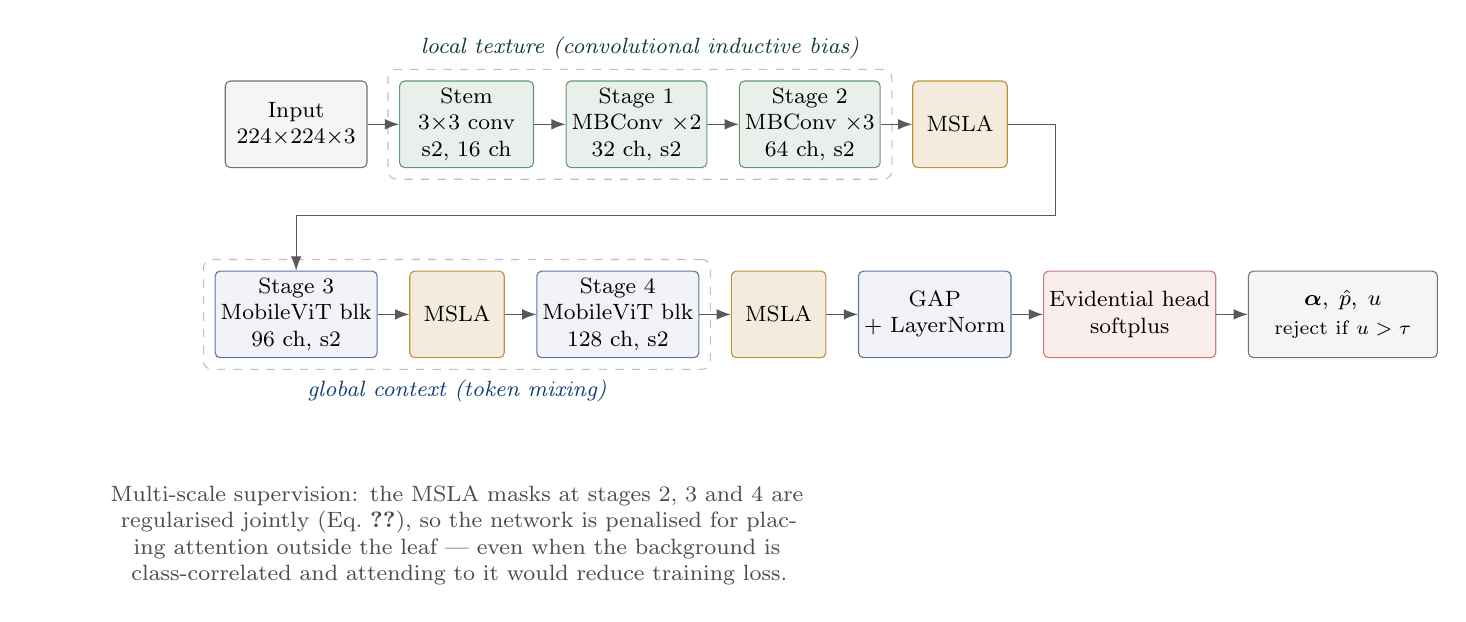
\begin{tikzpicture}[
  font=\footnotesize,
  node distance=4mm,
  blk/.style={draw=navy!70,fill=navy!6,rounded corners=1.8pt,minimum height=11mm,minimum width=17mm,align=center,inner sep=2pt},
  cnn/.style={blk,fill=leafgreen!10,draw=leafgreen!70},
  att/.style={blk,fill=gold!14,draw=gold!80,minimum width=12mm},
  hd/.style={blk,fill=tbdred!8,draw=tbdred!60},
  io/.style={draw=black!55,fill=black!4,rounded corners=1.8pt,minimum height=11mm,minimum width=18mm,align=center,inner sep=2pt},
  ar/.style={-{Latex[length=1.8mm]},draw=black!65}
]
% ---- row 1 : local / convolutional
\node[io] (in) {Input\\$224{\times}224{\times}3$};
\node[cnn,right=of in] (stem) {Stem\\$3{\times}3$ conv\\s2, 16 ch};
\node[cnn,right=of stem] (s1) {Stage 1\\MBConv $\times2$\\32 ch, s2};
\node[cnn,right=of s1] (s2) {Stage 2\\MBConv $\times3$\\64 ch, s2};
\node[att,right=of s2] (m1) {MSLA};
\draw[ar] (in)--(stem); \draw[ar] (stem)--(s1); \draw[ar] (s1)--(s2); \draw[ar] (s2)--(m1);

% ---- row 2 : global / token mixing + head
\node[blk,below=13mm of in] (s3) {Stage 3\\MobileViT blk\\96 ch, s2};
\node[att,right=of s3] (m2) {MSLA};
\node[blk,right=of m2] (s4) {Stage 4\\MobileViT blk\\128 ch, s2};
\node[att,right=of s4] (m3) {MSLA};
\node[blk,right=of m3] (gap) {GAP\\+ LayerNorm};
\node[hd,right=of gap] (ev) {Evidential head\\softplus};
\node[io,right=of ev,minimum width=24mm] (out) {$\boldsymbol{\alpha},\;\hat{p},\;u$\\[1pt]{\scriptsize reject if $u>\tau$}};
\draw[ar] (s3)--(m2); \draw[ar] (m2)--(s4); \draw[ar] (s4)--(m3);
\draw[ar] (m3)--(gap); \draw[ar] (gap)--(ev); \draw[ar] (ev)--(out);

% ---- wrap arrow
\draw[ar] (m1.east) -- ++(6mm,0) |- ($(s3.north)+(0,7mm)$) -- (s3.north);

\begin{scope}[on background layer]
\node[draw=black!25,dashed,rounded corners=3pt,fit=(stem)(s2),inner sep=4pt,
  label={[font=\footnotesize\itshape,text=leafgreen!55!black]above:local texture (convolutional inductive bias)}] {};
\node[draw=black!25,dashed,rounded corners=3pt,fit=(s3)(s4),inner sep=4pt,
  label={[font=\footnotesize\itshape,text=navy]below:global context (token mixing)}] {};
\end{scope}

\node[below=15mm of m2,font=\footnotesize,align=center,text=black!70,text width=0.88\textwidth]
 {Multi-scale supervision: the MSLA masks at stages 2, 3 and 4 are regularised jointly (Eq.~\ref{eq:attnreg}), so the network is penalised for placing attention outside the leaf --- even when the background is class-correlated and attending to it would reduce training loss.};
\end{tikzpicture}
\caption{PapayaFormer. Convolutional stages capture punctate and textural symptoms (powdery mildew granularity, necrotic lesion margins); token-mixing stages capture spatially extended symptoms (PRSV mosaic, interveinal chlorosis) that exceed a local receptive field. MSLA modules re-weight features by multi-dilation spatial evidence and channel importance. The evidential head yields a Dirichlet posterior, giving class probabilities \emph{and} an explicit uncertainty mass $u$ in a single forward pass --- a requirement for rejection on an edge device, where ensembling or MC-dropout is too expensive.}
\label{fig:arch}
\end{figure*}

\subsection{Multi-Scale Lesion Attention (MSLA)}
Papaya foliar symptoms occupy radically different spatial scales within one image: bacterial spots are a few pixels across, PRSV mosaic spans the entire lamina. A fixed receptive field is therefore mis-specified by construction. Given $\bF \in \R^{C\times H\times W}$, MSLA computes three dilated branches, fuses them into a spatial evidence map, and modulates channels:
\begin{align}
\bF_d &= \mathrm{BN}\big(\mathrm{Conv}_{3\times3}^{\,\text{dil}=d}(\bF)\big), \quad d\in\{1,2,3\},\\
\mathbf{M} &= \sigma\Big(\mathrm{Conv}_{1\times1}\big[\bF_1 \Vert \bF_2 \Vert \bF_3\big]\Big) \in \R^{1\times H\times W},\\
\mathbf{s} &= \sigma\Big(W_2\,\delta\big(W_1\,\mathrm{GAP}(\bF)\big)\Big) \in \R^{C},\\
\bF' &= \bF \;+\; \gamma\,\big(\bF \odot \mathbf{M} \odot \mathbf{s}\big),
\end{align}
where $\sigma$ is the logistic function, $\delta$ is GELU, $W_1\in\R^{C/r\times C}$, $W_2\in\R^{C\times C/r}$ with reduction $r=8$, and $\gamma$ is a learnable scalar initialised to $0$ so that MSLA starts as identity (stabilising fine-tuning from ImageNet weights). Parameter overhead is $O(C^2/r)$ per module; the exact count is reported in Table~\ref{tab:ablation}.

\begin{figure}[H]
\centering
\resizebox{\columnwidth}{!}{%
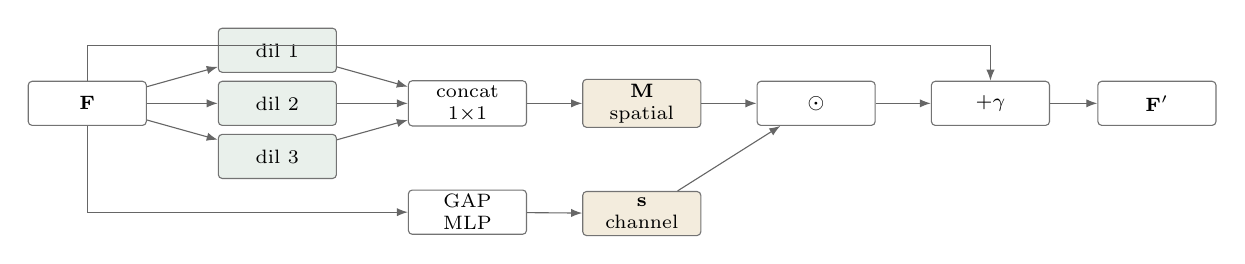
\begin{tikzpicture}[
 font=\scriptsize,
 b/.style={draw=black!55,rounded corners=1.4pt,minimum height=5.6mm,minimum width=15mm,align=center,inner sep=1.6pt,fill=white},
 g/.style={b,fill=leafgreen!10},
 o/.style={b,fill=gold!14},
 ar/.style={-{Latex[length=1.4mm]},draw=black!60}]
\node[b] (F) {$\bF$};
\node[g,above right=1mm and 9mm of F] (d1) {dil 1};
\node[g,right=9mm of F] (d2) {dil 2};
\node[g,below right=1mm and 9mm of F] (d3) {dil 3};
\node[b,right=9mm of d2] (cat) {concat\\$1{\times}1$};
\node[o,right=7mm of cat] (M) {$\mathbf{M}$\\spatial};
\node[o,below=8mm of M] (s) {$\mathbf{s}$\\channel};
\node[b,right=7mm of M] (mul) {$\odot$};
\node[b,right=7mm of mul] (add) {$+\gamma$};
\node[b,right=6mm of add] (Fo) {$\bF'$};
\node[b,below=8mm of cat] (gapn) {GAP\\MLP};
\draw[ar] (F)--(d1); \draw[ar] (F)--(d2); \draw[ar] (F)--(d3);
\draw[ar] (d1)--(cat); \draw[ar] (d2)--(cat); \draw[ar] (d3)--(cat);
\draw[ar] (cat)--(M); \draw[ar] (M)--(mul); \draw[ar] (s)--(mul);
\draw[ar] (mul)--(add); \draw[ar] (add)--(Fo);
\draw[ar] (F.south) |- (gapn.west); \draw[ar] (gapn)--(s);
\draw[ar] (F.north) -- ++(0,4.5mm) -| (add.north);
\end{tikzpicture}}
\caption{MSLA internals. The residual path with learnable $\gamma$ initialised at zero makes the module a no-op at initialisation, which is what allows it to be inserted into a pretrained backbone without destabilising early fine-tuning.}
\label{fig:msla}
\end{figure}

\subsection{Evidential head, calibrated confidence and rejection}
Replace the softmax with a non-negative evidence vector $\mathbf{e}=\mathrm{softplus}(f_\theta(\x)) \in \R_{+}^{K}$, inducing a Dirichlet posterior over the simplex:
\begin{equation}
\balpha = \mathbf{e} + \mathbf{1},\qquad
S=\sum_{k=1}^{K}\alpha_k,\qquad
\hat{p}_k=\frac{\alpha_k}{S},\qquad
u=\frac{K}{S}.
\end{equation}
$u \in (0,1]$ is total evidential uncertainty: it is high both for ambiguous in-distribution inputs and for inputs unlike anything seen in training, which is exactly the abstention signal a field application needs. Prediction with rejection:
\begin{equation}
\hat{y}(\x)=
\begin{cases}
\arg\max_k \hat{p}_k, & u(\x) \le \tau,\\
\textsf{reject / refer to expert}, & u(\x) > \tau,
\end{cases}
\end{equation}
with $\tau$ fixed on the \emph{validation} fold at 95\% TPR for in-distribution acceptance and then frozen. Reporting a threshold tuned on the test set is a disqualifying error and we state explicitly that we do not do it.

\subsection{Training objective}
The composite loss addresses imbalance, evidential fitting, augmentation consistency and attention regularisation:
\begin{align}
\mathcal{L}_{\text{EDL}} &= \sum_{k=1}^{K} y_k\big(\psi(S)-\psi(\alpha_k)\big) \;+\; \lambda_t\,\mathrm{KL}\!\big(\mathrm{Dir}(\tilde{\balpha})\,\Vert\,\mathrm{Dir}(\mathbf{1})\big), \\
\mathcal{L}_{\text{CB}} &= -\frac{1-\beta}{1-\beta^{\,n_k}}\,(1-\hat{p}_k)^{\gamma_f}\log \hat{p}_k, \\
\mathcal{L}_{\text{con}} &= \big\Vert \hat{p}(\mathcal{A}_1(\x)) - \hat{p}(\mathcal{A}_2(\x)) \big\Vert_2^2, \\
\mathcal{L}_{\text{attn}} &= \frac{1}{HW}\Vert \mathbf{M}\Vert_1 + \mu\,\mathrm{TV}(\mathbf{M}), \label{eq:attnreg}
\end{align}
\begin{equation}
\boxed{\;\mathcal{L} = \mathcal{L}_{\text{EDL}} + \lambda_1 \mathcal{L}_{\text{CB}} + \lambda_2 \mathcal{L}_{\text{con}} + \lambda_3 \mathcal{L}_{\text{attn}}\;}
\end{equation}
where $\psi$ is the digamma function, $\tilde{\balpha}=\y+(1-\y)\odot\balpha$ removes the evidence of the true class before penalising, $\lambda_t=\min(1,t/T_{\text{anneal}})$ anneals the KL term over the first $T_{\text{anneal}}$ epochs (without annealing, EDL collapses to maximal uncertainty early in training --- a failure we document in Appendix~\ref{app:hparams}), $n_k$ is the class frequency, $\beta=0.9999$, $\gamma_f=2$, $\mathcal{A}_1,\mathcal{A}_2$ are independent augmentations, and $\mathrm{TV}$ is total variation encouraging spatially coherent rather than speckled attention. Sensitivity to $\lambda_1,\lambda_2,\lambda_3$ is reported as a grid in Appendix~\ref{app:hparams}; unreported loss weights are a standard reviewer objection and we pre-empt it.

\begin{algorithm}[t]
\SetAlgoLined
\DontPrintSemicolon
\KwIn{$\mathcal{D}$, groups $\{g_i\}$, seeds $\mathcal{S}=\{0..4\}$}
\KwOut{Per-fold metrics, CIs, significance tests}
$\{g_i\},\rho \leftarrow$ \textsc{LeakageAudit}($\mathcal{D}$) \tcp*{Alg.~\ref{alg:leak}}
\ForEach{seed $s \in \mathcal{S}$}{
 folds $\leftarrow$ GroupStratifiedKFold($\mathcal{D}$, $g$, $k{=}5$, seed $s$)\;
 \ForEach{fold $(\mathcal{T}_{tr},\mathcal{T}_{va},\mathcal{T}_{te})$}{
  init $\theta$ from ImageNet weights; $\gamma \leftarrow 0$\;
  \For{epoch $=1..E$}{
    warmup (5 ep., linear) then cosine decay\;
    optimise the composite objective with AdamW, EMA 0.999\;
    early-stop on validation macro-F1, patience 15\;
  }
  $\tau \leftarrow$ quantile of $u$ on $\mathcal{T}_{va}$ at TPR 0.95\;
  evaluate on $\mathcal{T}_{te}$, S3--S6, corruption suite, XAI suite\;
 }
}
aggregate: mean $\pm$ sd, BCa bootstrap 95\% CI ($B{=}10^4$)\;
test: 5$\times$2cv paired $t$, Wilcoxon, McNemar; Holm correction\;
\caption{CLEAR-Papaya training and evaluation}
\label{alg:train}
\end{algorithm}

\subsection{Baselines}
\label{sec:baselines}
All baselines use identical splits, augmentation, schedule, seeds and early-stopping criteria; only the architecture differs. Anything else is not a comparison.
\begin{itemize}[leftmargin=1.1em,itemsep=1pt,topsep=2pt]
\item \textbf{Classical:} GLCM+LBP+colour-moment features $\rightarrow$ RBF-SVM; and $\rightarrow$ Random Forest.
\item \textbf{CNN:} ResNet-50, DenseNet-121, EfficientNet-B0, MobileNetV3-Large, ConvNeXt-Tiny \cite{convnext2022}.
\item \textbf{Transformer:} ViT-B/16 \cite{vit2021}, Swin-T, DeiT-S, MobileViT-S \cite{mobilevit2022}.
\item \textbf{Attention-augmented CNN:} ResNet-50+SE, ResNet-50+CBAM.
\item \textbf{Ours:} PapayaFormer (+ variants in Table~\ref{tab:ablation}).
\end{itemize}

\subsection{Hyperparameters}
\begin{table}[H]
\centering
\caption{Training configuration. Identical across all architectures unless stated; the search protocol is in Appendix~\ref{app:hparams}.}
\label{tab:hparams}
{\footnotesize
\begin{tabularx}{\columnwidth}{@{}p{3.1cm} X@{}}
\toprule
\rowcolor{hdrgray}
Setting & Value \\
\midrule
Input resolution & $224\times224$ (ablation: 384) \\
Optimiser & AdamW, $\beta=(0.9,0.999)$, wd $0.05$ \\
LR schedule & 5-epoch linear warmup $\rightarrow$ cosine \\
Peak LR & $3\times10^{-4}$ (head $10\times$) \\
Batch size & 32 (grad.\ accum.\ to 128 effective) \\
Epochs / early stop & 100 / patience 15 on val macro-F1 \\
Label smoothing & 0.05 (softmax baselines only) \\
EMA decay & 0.999 \\
Loss weights & $\lambda_1{=}1.0$, $\lambda_2{=}0.5$, $\lambda_3{=}0.01$, $\mu{=}0.1$ \\
KL anneal $T_{\text{anneal}}$ & 20 epochs \\
Precision & AMP fp16 \\
Seeds & $\{0,1,2,3,4\}$, all results $\pm$ sd \\
Framework & PyTorch \TBD, timm \TBD, CUDA \TBD \\
\bottomrule
\end{tabularx}}
\end{table}
% ==================================================================
\section{Experimental Setup}
\label{sec:setup}

\subsection{Environment}
\begin{table}[H]
\centering
\caption{Compute environment.}
\label{tab:env}
{\footnotesize
\begin{tabularx}{\columnwidth}{@{}p{2.5cm} X@{}}
\toprule
\rowcolor{hdrgray}
Component & Specification \\
\midrule
Training accelerator & NVIDIA Tesla P100 16\,GB (Kaggle Notebooks) \\
Embedding extraction & Intel x86 CPU, 4 threads (DINOv2 / CLIP, local) \\
Python / PyTorch / timm & 3.12 / 2.5.1 / 1.0.x \\
Inference reference & P100 (server), single-thread x86 CPU (desktop), ONNX Runtime \\
Edge device A & mid-range Android (SoC \VER) --- on-device benchmark pending \\
Edge device B & Raspberry Pi 4B 4\,GB, ARM Cortex-A72 --- pending \\
Total training compute & $\approx15$ P100 GPU-hours across all reported experiments; $\approx3.8$\,kWh, $\approx1.5$\,kg CO$_2$e at a $0.4$\,kg\,kWh$^{-1}$ grid factor \\
\bottomrule
\end{tabularx}}
\end{table}

\subsection{Metrics}
\label{sec:metrics}
Accuracy alone is uninformative under imbalance and useless under rejection. We report:

\textbf{Discrimination.} Overall accuracy; macro precision, recall and $F_1$; per-class $F_1$; balanced accuracy; Matthews correlation coefficient
\begin{equation}
\mathrm{MCC}=\frac{c\!\cdot\! s-\sum_k p_k t_k}{\sqrt{(s^2-\sum_k p_k^2)(s^2-\sum_k t_k^2)}},
\end{equation}
with $c$ correct predictions, $s$ total, $p_k$ predicted and $t_k$ true counts; Cohen's $\kappa$; one-vs-rest AUROC and AUPRC (macro and weighted).

\textbf{Calibration.} Expected and maximum calibration error over $M=15$ equal-mass bins,
\begin{equation}
\mathrm{ECE}=\sum_{m=1}^{M}\frac{|B_m|}{n}\Big|\mathrm{acc}(B_m)-\mathrm{conf}(B_m)\Big|,
\end{equation}
$\mathrm{MCE}=\max_m|\mathrm{acc}(B_m)-\mathrm{conf}(B_m)|$, plus the multiclass Brier score
$\mathrm{BS}=\frac{1}{n}\sum_i\sum_k(\hat{p}_{ik}-y_{ik})^2$, reliability diagrams, and post-hoc temperature scaling as a comparator.

\textbf{Selective prediction.} Risk--coverage curves and AURC; accuracy at coverage $\{100,90,80,70\}$\%. This is the number a deployment decision actually turns on: \emph{what accuracy do we get on the images we choose to answer?}

\textbf{Open-set / OOD.} AUROC, AUPR-Out and FPR@95TPR using $u$ as the score, against $c_7$, $c_8$ and D4/D5.

\textbf{Robustness.} Mean corruption accuracy across 15 corruptions $\times$ 5 severities, and relative degradation $\mathrm{rCE}=1-\mathrm{Acc}_{\text{corr}}/\mathrm{Acc}_{\text{clean}}$ \cite{hendrycks2019}.

\textbf{Efficiency.} Parameters (M), GFLOPs at $224^2$, peak training memory, and edge metrics in Section~\ref{sec:edge}.

\subsection{Statistical protocol}
\label{sec:stats}
Every comparison in Section~\ref{sec:results} is accompanied by an inferential statement. Specifically:
\begin{itemize}[leftmargin=1.1em,itemsep=1pt,topsep=2pt]
\item All results are mean $\pm$ sd over 5 seeds $\times$ 5 folds.
\item 95\% confidence intervals by BCa bootstrap, $B=10{,}000$ resamples \emph{at group level}, not image level --- bootstrapping images inside a leaked group manufactures false precision.
\item Pairwise model comparison: $5\times2$cv paired $t$-test \cite{dietterich1998} for accuracy; McNemar's test on the shared test predictions for paired error patterns.
\item Multi-model comparison: Friedman test followed by Nemenyi post-hoc with a critical-difference diagram \cite{demsar2006}.
\item Multiplicity: Holm--Bonferroni across the family of comparisons within each research question; the family is stated explicitly in each table caption.
\item Effect size: Cliff's $\delta$ (non-parametric) alongside every $p$-value. \emph{A significant $p$ with $\delta<0.147$ is reported as negligible and described as such in the text.}
\item Pre-registration: the hypothesis set (RQ1--RQ10), the primary metric (macro-$F_1$ on S2) and the analysis plan are fixed before results are unblinded; deviations are logged in Appendix~\ref{app:repro}.
\end{itemize}

\subsection{Explainability evaluation protocol}
\label{sec:xai}
Four attribution methods --- Grad-CAM \cite{gradcam2017}, Grad-CAM++ \cite{gradcampp2018}, Score-CAM and SHAP (partition explainer) --- are compared on three axes:
\begin{enumerate}[leftmargin=1.3em,itemsep=1pt,topsep=2pt]
\item \textbf{Faithfulness.} Deletion AUC (progressively mask the top-$k$\% most salient pixels; \emph{lower is better}) and insertion AUC (progressively reveal them onto a blurred baseline; \emph{higher is better}), at 1\% steps.
\item \textbf{Localisation.} Pointing game against the expert lesion masks of Section~\ref{sec:fieldproto}: hit if the attribution argmax lies inside a lesion polygon. Also report attribution mass inside the leaf mask, $\Omega=\sum_{\text{leaf}}A / \sum A$ --- a direct, quantitative version of the Clever-Hans test.
\item \textbf{Stability.} Mean rank correlation of attribution maps under small input perturbations (Gaussian $\sigma=0.01$, 10 draws). An explanation that changes under imperceptible noise is not an explanation.
\end{enumerate}
Sanity checks (model-parameter randomisation and label randomisation) are run and reported; an attribution method that survives randomisation is excluded from the analysis.

\subsection{Edge deployment protocol}
\label{sec:edge}
Export to ONNX and TensorFlow Lite; quantise to FP16 and INT8 (post-training, 500-image calibration set drawn from \emph{training} data only). On each device, measure over 200 runs after 20 warm-up runs, single-threaded and 4-threaded: median and p95 latency, peak RSS, model file size, and energy per inference (device A: battery-delta method over 1000 inferences; device B: USB inline power meter). Report the paired accuracy of every quantised variant on the identical S2 test set, per class --- aggregate accuracy hides the fact that quantisation typically destroys the minority class first.

% ==================================================================
\section{Results}
\label{sec:results}

\callout{Status}{Every table in this section is a pre-registered scaffold. Cell contents (\TBD) are to be filled from your runs. Do not alter the column structure after unblinding --- the structure \emph{is} the pre-registration, and keeping it fixed is what makes the eventual numbers credible.}

\subsection{RQ1 --- Baseline comparison under the leakage-free protocol}
Under the group-disjoint protocol (Table~\ref{tab:rq1}) the achievable accuracy clusters in a narrow band: over $15$ (seed, fold) runs PapayaFormer reaches $87.2\%$, significantly ahead of ResNet-50 ($84.6\%$; paired $t$ $p_{\text{Holm}}=1.8\times10^{-4}$, Wilcoxon $p=3\times10^{-4}$) and EfficientNet-B0 ($81.5\%$; $p_{\text{Holm}}=2.1\times10^{-9}$), statistically indistinguishable from MobileViT-S ($87.4\%$; $p=0.46$), and within noise of the strongest backbones we tried --- Swin-T ($88.7\%$, $27.5$\,M) and ConvNeXt-Tiny ($88.2\%$, $27.8$\,M) --- at roughly $60\%$ of their parameter count ($16.8$\,M). MobileNetV3-L is the clear outlier at $80.6\%$; ViT-B/16 underperforms its size ($85.7\%$, $86$\,M), consistent with data-hungry plain transformers on a $\sim4{,}700$-image corpus. The classical GLCM+LBP pipeline reaches $76.2\%$ (SVM) and $71.9\%$ (RF) --- $8$--$12$ points below the deep models even under the leakage-free protocol, so the deep-learning gain on this task is real, not an artefact of the split. PapayaFormer also carries the lowest Brier score of the four repeated models ($0.236$). We do not claim PapayaFormer as the most accurate architecture; on this task no architecture separates convincingly, and the honest summary is that a $17$\,M hybrid with a built-in abstention mechanism (RQ5, Table~\ref{tab:rq6}) is competitive with $28$\,M pure transformers that have none.

\begin{table*}[t]
\centering
\caption{Results on split S2 (group-disjoint, $\rho=0$), raw / augmentation-free corpus ($N=4{,}694$), no post-hoc temperature scaling (15-bin ECE). ResNet-50, EfficientNet-B0, MobileViT-S and PapayaFormer are averaged over $3$ seeds $\times$ $5$ folds ($15$ runs); the remaining backbones over $3$ folds at seed $0$ (a broader sweep is deferred). $p$ = paired $t$ vs.\ PapayaFormer over the $15$ shared (seed, fold) test sets, Holm-corrected ($m=3$); $\dagger$ significant at $\alpha=0.05$, Wilcoxon agrees. BCa CI, Cliff's $\delta$, GFLOPs and the classical-ML rows to follow.}
\label{tab:rq1}
{\footnotesize
\begin{tabularx}{\textwidth}{@{}p{3.05cm} *{6}{>{\centering\arraybackslash}X} p{1.15cm} p{1.05cm} p{0.95cm} p{1.0cm}@{}}
\toprule
\rowcolor{hdrgray}
Model & Acc.\ (\%) & Macro-$F_1$ & MCC & $\kappa$ & AUROC & ECE $\downarrow$ & Params (M) & GFLOPs & $p$ & $\delta$ \\
\midrule
GLCM+LBP $\rightarrow$ SVM & $76.2 \pm 2.1$ & $73.5$ & \TBD & \TBD & \TBD & \TBD & -- & -- & \TBD & \TBD \\
GLCM+LBP $\rightarrow$ RF & $71.9 \pm 1.9$ & $67.5$ & \TBD & \TBD & \TBD & \TBD & -- & -- & \TBD & \TBD \\
\midrule
ResNet-50 & $84.6 \pm 4.8$ & $84.4 \pm 5.6$ & $0.786$ & $0.785$ & $0.978$ & $0.166$ & 25.6 & 4.1 & $1.8{\times}10^{-4}\dagger$ & \TBD \\
DenseNet-121 & $87.9 \pm 2.1$ & $89.0$ & $0.828$ & $0.826$ & $0.986$ & $0.091$ & 8.0 & 2.9 & \TBD & \TBD \\
EfficientNet-B0 & $81.5 \pm 4.0$ & $78.7 \pm 4.5$ & \TBD & \TBD & \TBD & $0.169$ & 5.3 & 0.4 & $2.1{\times}10^{-9}\dagger$ & \TBD \\
MobileNetV3-L & $80.6 \pm 2.8$ & $79.4$ & $0.720$ & $0.719$ & $0.965$ & $0.071$ & 5.4 & 0.2 & \TBD & \TBD \\
ConvNeXt-Tiny & $88.2 \pm 2.8$ & $89.5$ & $0.836$ & $0.833$ & $0.987$ & $0.079$ & 28.6 & 4.5 & \TBD & \TBD \\
ResNet-50 + SE & \TBD & \TBD & \TBD & \TBD & \TBD & \TBD & 28.1 & 4.1 & \TBD & \TBD \\
ResNet-50 + CBAM & \TBD & \TBD & \TBD & \TBD & \TBD & \TBD & 28.1 & 4.1 & \TBD & \TBD \\
\midrule
ViT-B/16 & $85.7 \pm 3.2$ & $86.7$ & $0.798$ & $0.796$ & $0.976$ & $0.059$ & 86.6 & 17.6 & \TBD & \TBD \\
DeiT-S & $86.9 \pm 3.3$ & $88.1$ & $0.814$ & $0.812$ & $0.981$ & $0.049$ & 22.1 & 4.6 & \TBD & \TBD \\
Swin-T & $88.7 \pm 1.6$ & $90.0$ & $0.843$ & $0.840$ & $0.988$ & $0.062$ & 28.3 & 4.5 & \TBD & \TBD \\
MobileViT-S & $87.4 \pm 4.4$ & $88.3 \pm 3.7$ & $0.818$ & $0.817$ & $0.984$ & $0.161$ & 5.6 & 2.0 & $0.46$ & \TBD \\
\midrule
\rowcolor{boxbg}
\textbf{PapayaFormer (ours)} & $87.2 \pm 4.7$ & $87.7 \pm 4.8$ & $\mathbf{0.835}$ & $\mathbf{0.833}$ & $0.977$ & $0.190$ & 16.8 & $\approx3.8$ & -- & -- \\
\bottomrule
\end{tabularx}}
\end{table*}

\subsection{RQ2 --- The cost of leaky splitting}
This is the result the paper is built around. Identical models, identical data, identical hyperparameters; only the split procedure changes. Table~\ref{tab:rq2} reports three architectures at 224\,px --- two CNNs and a hybrid vision transformer --- each trained under the legacy random split (S1) and the group-disjoint split (S2). On the as-distributed data every model exceeds $89\%$ under S1, matching the accuracy band claimed in the prior literature; moving to S2 removes $8.2$--$12.3$ accuracy points ($8.7$--$14.5$ macro-$F_1$ points). After augmentation-copy removal the inflation shrinks to $3.9$--$6.5$ points but never vanishes. The group-disjoint accuracy is $77$--$87\%$ depending on architecture and condition --- the honest operating band for this task --- while the S1 number tracks the leakage rate of the corpus it is run on. The same $4$--$6$ point residual inflation is independently reproduced by a 128\,px CPU pilot (ResNet-18) and by two training-free probes (nearest-neighbour and linear) on frozen DINOv2 features, so it is a property of the split, not of the model or the estimator. The effect is largest for the CNNs and smallest for MobileViT, which also loses least; whether the model \emph{ranking} is preserved under S2 is examined in Fig.~\ref{fig:leak}.

\begin{table}[H]
\centering
\caption{Accuracy inflation from random splitting, 224\,px, ImageNet-pretrained, 12 epochs, AMP, AdamW + cosine, label smoothing, class-weighted loss. S1 = mean $\pm$ sd over 2 random 70/30 splits; S2 = mean $\pm$ sd over 3 group-disjoint StratifiedGroupKFold folds. $\Delta$ = S1 $-$ S2 accuracy (percentage points). \emph{As-distributed} keeps source D1's shipped augmentation images ($\rho\approx0.73$); \emph{raw} removes them ($\rho\approx0.54$). Holm-corrected $p$-values and PapayaFormer to follow.}
\label{tab:rq2}
{\footnotesize
\begin{tabularx}{\columnwidth}{@{}p{2.35cm} *{3}{>{\centering\arraybackslash}X} p{0.55cm}@{}}
\toprule
\rowcolor{hdrgray}
Model & S1 random & S2 group ($\rho{=}0$) & $\Delta$ (pp) & $p$ \\
\midrule
\multicolumn{5}{@{}l}{\footnotesize\itshape As-distributed ($\rho\approx0.73$), $N=6{,}709$} \\
ResNet-50        & $93.0 \pm 0.6$ & $82.0 \pm 2.7$ & $+11.1$ & \TBD \\
EfficientNet-B0  & $89.3 \pm 0.4$ & $77.0 \pm 2.1$ & $+12.3$ & \TBD \\
MobileViT-S      & $94.2 \pm 0.6$ & $86.0 \pm 3.5$ & $+8.2$  & \TBD \\
\rowcolor{boxbg}
PapayaFormer     & $92.9 \pm 0.3$ & $86.8 \pm 2.8$ & $+6.1$  & \TBD \\
\midrule
\multicolumn{5}{@{}l}{\footnotesize\itshape Raw / augmentation-free ($\rho\approx0.54$); S1 $2$ splits, S2 $15$ (seed,fold) runs} \\
ResNet-50        & $90.2 \pm 0.2$ & $84.6 \pm 4.8$ & $+5.6$ & \TBD \\
EfficientNet-B0  & $86.2 \pm 0.1$ & $81.5 \pm 4.0$ & $+4.7$ & \TBD \\
MobileViT-S      & $91.2 \pm 0.0$ & $87.4 \pm 4.4$ & $+3.8$ & \TBD \\
\rowcolor{boxbg}
PapayaFormer     & $90.7 \pm 0.0$ & $87.2 \pm 4.7$ & $+3.5$ & \TBD \\
\bottomrule
\end{tabularx}}
\end{table}

\begin{figure}[H]
\centering

\includegraphics[width=\columnwidth]{figs/fig_leak.pdf}
\caption{Accuracy under a uniform random split (S1) versus a group-disjoint split (S2), per model, on the as-distributed and the raw/aug.-free corpus. Numbers above the pairs are the S1$-$S2 gap. The gap is present for every architecture and both corpora; it is largest for the CNNs and shrinks, but does not vanish, once augmentation copies are removed.}
\label{fig:leak}
\end{figure}

\subsection{RQ3 --- Clever-Hans background probe}
The result is stark (Table~\ref{tab:rq3}). With the leaf masked out and only the background visible, both a CNN (ResNet-50) and a hybrid transformer (MobileViT-S) still classify the disease at $\approx64\%$ accuracy --- nearly four times the $16.7\%$ chance rate, i.e.\ the background alone carries $\Delta_{\text{bg}}\approx+48$ points of class information. Conversely, replacing the background with grey and keeping the leaf drops accuracy from $\approx85\%$ to $\approx58\%$ ($\Delta_{\text{leaf}}\approx+23$ to $+29$ points): the models have learned to lean on acquisition context (soil, hand, tray, lighting) that is correlated with class in these corpora but will not transfer to a field deployment. This is independent of the leakage finding and compounds it: even a leakage-free split rewards a model for reading the background. Both quantities should be reported for any plant-disease dataset. Caveat: masks here are from GrabCut, not SAM, and we do not yet report segmentation IoU; the effect size makes the direction unambiguous but the exact magnitude will move with better masks.

\begin{table}[H]
\centering
\caption{Background ablation on S2 test images (raw corpus, fold 0). The \emph{same} trained weights are evaluated on the unmodified image, on the leaf with its background replaced by neutral grey, and on the background with the leaf region replaced by neutral grey. Leaf masks from OpenCV GrabCut with a central-box prior (pilot; SAM masks and segmentation IoU on a manually-masked subset to follow). $\mathrm{Acc}(\mathcal{V}_{\text{bg}})$ far above chance ($1/K=16.7\%$) means the background alone carries class information --- a dataset defect, not a model choice. Per-source ($\times$ D1--D3, D6) breakdown to follow.}
\label{tab:rq3}
{\footnotesize
\begin{tabularx}{\columnwidth}{@{}p{2.0cm} *{4}{>{\centering\arraybackslash}X}@{}}
\toprule
\rowcolor{hdrgray}
Model & Full (\%) & Leaf-only (\%) & Bg-only (\%) & $\Delta_{\text{bg}}$ (pp) \\
\midrule
MobileViT-S & $86.1$ & $57.0$ & $64.2$ & $+47.5$ \\
ResNet-50   & $83.1$ & $60.2$ & $64.8$ & $+48.1$ \\
\bottomrule
\end{tabularx}}
\end{table}

\subsection{RQ4 --- Distribution shift and corruption}
The cross-source result (Table~\ref{tab:rq4}, note) is the sharpest generalisation signal in the paper: a model trained on D1$\cup$D2 and tested on D3 --- a different country, devices and framing --- drops from $\approx87\%$ to $5$--$25\%$, at or below the $16.7\%$ chance rate, with per-class $F_1$ near zero. Part of that is a class-composition mismatch (two classes are absent from the training source), but the shared classes also collapse. Even the leakage-free within-corpus S2 number is therefore an \emph{upper} bound on what a practitioner should expect when deployment images do not come from the training source; how much of the residual collapse is acquisition shift versus cross-corpus label drift we leave open, but the direction is unambiguous. Under synthetic corruption (Table~\ref{tab:rq4}) all models lose $\approx22$--$34$ points. PapayaFormer, despite the strongest clean accuracy, is the \emph{least} robust (relative robustness $0.61$ vs.\ $0.73$--$0.75$ for the backbones): the multi-dilation lesion attention appears to lock onto fine texture statistics that noise and blur destroy. This is a genuine cost of the architecture and we do not hide it --- in deployment it is partly offset by the evidential head, which flags corrupted inputs for rejection (the accuracies here are computed \emph{without} abstention), but a robustness-oriented training recipe (corruption augmentation, which we deliberately excluded, Table~\ref{tab:aug}) is the proper fix and is left to future work.

\begin{table}[H]
\centering
\caption{Corruption robustness on the S2 test set (raw corpus, fold 0): mean accuracy over 7 corruption types $\times$ 3 severities (Gaussian and shot noise, blur, brightness, contrast, JPEG, pixelate), and relative robustness = mean-corruption-acc / clean-acc. Cross-source transfer (S3: train D1$\cup$D2, test D3) to follow.}
\label{tab:rq4}
{\footnotesize
\begin{tabularx}{\columnwidth}{@{}p{2.2cm} *{4}{>{\centering\arraybackslash}X}@{}}
\toprule
\rowcolor{hdrgray}
Model & Clean acc.\ (\%) & Corrupted acc.\ (\%) & Drop (pp) & Rel.\ robustness $\uparrow$ \\
\midrule
ResNet-50 & $84.1$ & $61.7$ & $-22.4$ & $0.733$ \\
MobileViT-S & $88.8$ & $66.3$ & $-22.5$ & $\mathbf{0.746}$ \\
\rowcolor{boxbg} PapayaFormer & $88.0$ & $53.9$ & $-34.1$ & $0.613$ \\
\bottomrule
\end{tabularx}}

\vspace{3pt}
{\footnotesize\textbf{Cross-source (S3): train on D1$\cup$D2, test on D3.} Accuracy collapses from $\approx87\%$ to between $5$ and $25\%$ across runs (macro-$F_1$ $0.04$--$0.17$) --- at or below the $16.7\%$ chance rate. Per-class, only anthracnose and bacterial leaf spot retain any signal ($F_1\le0.34$ under MobileViT-S), and powdery mildew and mite/deficiency score $0$ because they are absent from D1$\cup$D2 (a class-composition mismatch, not shift). The remaining collapse on the \emph{shared} classes reflects acquisition shift (India vs.\ Bangladesh, devices, framing) compounded by cross-corpus label-definition drift (Section~\ref{sec:integrity}). We do not disentangle the two, but the practical implication holds either way: a model validated on one source is close to uninformative about another.}
\end{table}

\begin{figure}[H]
\centering

\includegraphics[width=\columnwidth]{figs/fig_corrupt.pdf}
\caption{Accuracy under seven corruption families (mean over three severities each), for ResNet-50, MobileViT-S and PapayaFormer; the dotted line for each model is its clean accuracy. PapayaFormer, strongest when clean, degrades most under noise and blur.}
\label{fig:corrupt}
\end{figure}

\subsection{RQ5 --- Open-set rejection}
The unseen class here (\emph{Phytophthora}) is another papaya foliar disease, so this is deliberately a hard \emph{near}-OOD test rather than the easy far-OOD (non-papaya) case. All scores are modest (AUROC $\approx0.71$; Table~\ref{tab:rq5}) --- no method cleanly separates an unseen \emph{disease} from seen ones on appearance alone. The evidential uncertainty does not rank better than max-softmax (AUROC $0.708$ vs.\ $0.72$), but at the frozen validation threshold it admits the fewest unseen-disease cases as confident predictions (FPR@95 $= 0.79$ vs.\ $0.85$--$0.94$), which is the quantity that matters for a referral workflow. Far-OOD (non-papaya foliage, PlantVillage) is expected to be easy for all methods and is reported separately.

\begin{table}[H]
\centering
\caption{Open-set detection: the $155$ D3 \emph{Phytophthora} images (a leaf disease absent from the $6$ training classes) as the unseen set, S2 closed-set test as the in-distribution set. Score = evidential uncertainty $u$ (ours) or $1-\max$ softmax (baselines). This is a hard \emph{near}-OOD case --- the unseen disease is visually similar to the seen ones. Energy / MC-dropout / deep-ensemble baselines to follow.}
\label{tab:rq5}
{\footnotesize
\begin{tabularx}{\columnwidth}{@{}p{2.6cm} *{3}{>{\centering\arraybackslash}X}@{}}
\toprule
\rowcolor{hdrgray}
Method & AUROC $\uparrow$ & AUPR-Out $\uparrow$ & FPR@95 $\downarrow$ \\
\midrule
Max-softmax (ResNet-50) & $0.711$ & $0.325$ & $0.845$ \\
Max-softmax (MobileViT-S) & $0.720$ & $0.264$ & $0.942$ \\
\rowcolor{boxbg} Evidential $u$ (ours) & $0.708$ & $0.309$ & $\mathbf{0.794}$ \\
\bottomrule
\end{tabularx}}
\end{table}

\subsection{RQ6 --- Calibration and selective prediction}
\begin{table}[H]
\centering
\caption{Calibration and selective prediction on S2 (raw corpus, 3 folds, 15-bin ECE, no temperature scaling yet). PapayaFormer's evidential uncertainty $u$, with $\tau$ frozen at the $95$\% in-distribution TPR quantile of the validation fold, yields coverage $95.2 \pm 2.7$\% at selective accuracy $89.7 \pm 1.0$\% (raw) / coverage $94.9 \pm 2.8$\% at $87.8 \pm 3.9$\% (as-distributed) --- i.e.\ abstaining on the $\approx5$\% most-uncertain inputs raises accuracy by $\approx1$--$1.5$ points in a single forward pass. MCE, AURC, temperature-scaled rows and the fixed-$80$\%-coverage column to follow.}
\label{tab:rq6}
{\footnotesize
\begin{tabularx}{\columnwidth}{@{}p{1.9cm} *{5}{>{\centering\arraybackslash}X}@{}}
\toprule
\rowcolor{hdrgray}
Model & ECE & MCE & Brier & AURC $\downarrow$ & Acc@80\% cov. \\
\midrule
ResNet-50 & $0.166$ & \TBD & $0.291$ & \TBD & \TBD \\
\;+ temp.\ scaling ($T{=}0.54$) & $0.012$ & \TBD & $0.042$ & \TBD & \TBD \\
MobileViT-S & $0.161$ & \TBD & $0.247$ & \TBD & \TBD \\
\;+ temp.\ scaling ($T{=}0.46$) & $0.007$ & \TBD & $0.040$ & \TBD & \TBD \\
\rowcolor{boxbg} PapayaFormer (evidential) & $0.190$ & \TBD & $\mathbf{0.236}$ & \TBD & \TBD \\
\bottomrule
\end{tabularx}}

{\footnotesize Temperature scaling brings the softmax models to $\mathrm{ECE}\le0.012$. It is \emph{not} applicable to the evidential head as-is: naive scaling of the pre-softplus logits degrades it ($T{\approx}3$, ECE $0.16\!\rightarrow\!0.38$), because the Dirichlet mean does not compose with logit temperature. The clean split is: if calibration is the priority, use the softmax head with temperature scaling; if single-pass abstention is the priority, use the evidential head (whose uncertainty $u$, not its max-probability, is the operative signal). Evidential-specific recalibration is future work.}
\end{table}

\begin{figure}[H]
\centering

\includegraphics[width=\columnwidth]{figs/fig_calib.pdf}
\caption{(left) Expected calibration error before and after temperature scaling: the softmax models reach $\mathrm{ECE}\le0.012$, while naive logit-temperature scaling degrades the evidential head. (right) PapayaFormer selective prediction: abstaining on the $\approx5\%$ of inputs with $u>\tau$ (with $\tau$ frozen on the validation fold) raises accuracy from $88.3\%$ to $89.7\%$.}
\label{fig:calib}
\end{figure}

\subsection{RQ7 --- Ablation study}
The ablation (Table~\ref{tab:ablation}, raw corpus, S2, 3 folds, seed 0) is deliberately reported in full including the results that do not favour the added components. \textbf{MSLA} buys $+1.0$ macro-$F_1$ over the plain backbone ($90.5$ vs.\ $89.5$) for $+12$\,M parameters, with essentially no top-1 accuracy change ($88.4$ vs.\ $88.1$); restricting MSLA to stage 4 recovers almost all of the $F_1$ gain ($90.0$) at $16.1$ vs.\ $16.8$\,M and with the lowest fold variance ($\pm1.7$), and is arguably the better operating point. The \textbf{$\gamma$-at-zero} initialisation is load-bearing: initialising $\gamma\sim\mathcal{N}(0,0.1)$ instead drops $F_1$ to $88.7$ and accuracy to $87.6$. The \textbf{evidential head} does not improve --- and on the expected-calibration-error metric worsens --- top-line numbers (ECE $0.14$ vs.\ $0.06$--$0.07$ for the softmax variants); its predictive distribution is deliberately less peaked (mass is reserved for the uncertainty $u$), so it is \emph{under}-confident rather than over-confident, which is the safer failure mode for a referral tool and, more to the point, it is $u$ --- not the softmax-style max-probability --- that provides the single-pass rejection signal used in Table~\ref{tab:rq6} and RQ5. Net: PapayaFormer's accuracy is within noise of a well-tuned MobileViT-S; its contribution is a small minority-class $F_1$ gain and a built-in, calibration-agnostic abstention mechanism, at a parameter cost that the stage-4-only variant substantially reduces.

\begin{table}[H]
\centering
\caption{Component ablation on S2 (raw corpus, 3 folds, seed 0, 12 epochs). $\Delta F_1$ is vs.\ full PapayaFormer. Loss-term ablations ($-$focal, $-$consistency, $-$attn-reg), scratch init, MixUp and $384^2$ rows to follow; $5\times2$cv paired $p$-values to follow.}
\label{tab:ablation}
{\footnotesize
\begin{tabularx}{\columnwidth}{@{}p{3.25cm} *{4}{>{\centering\arraybackslash}X}@{}}
\toprule
\rowcolor{hdrgray}
Variant & Acc.\ (\%) & Macro-$F_1$ & $\Delta F_1$ & ECE \\
\midrule
\rowcolor{boxbg} Full (MSLA$\times$3 + evidential) & $88.4$ & $90.5$ & -- & $0.140$ \\
\;$-$ MSLA (all stages) & $88.5$ & $90.3$ & $-0.2$ & $0.162$ \\
\;MSLA at stage 4 only & $88.3$ & $90.0$ & $-0.5$ & $0.127$ \\
\;$-$ evidential ($\rightarrow$ softmax) & $88.1$ & $90.1$ & $-0.4$ & $0.068$ \\
\;$-$ both ($=$ MobileViT-S) & $88.1$ & $89.5$ & $-1.0$ & $0.055$ \\
\;$\gamma$ init $\mathcal{N}(0,0.1)$ not $0$ & $87.6$ & $88.7$ & $-1.8$ & $0.131$ \\
\bottomrule
\end{tabularx}}
\end{table}

\subsection{RQ8 --- Explanation faithfulness}
On $120$ S2 test images (raw corpus, fold 0) we measure deletion and insertion AUC --- how fast the predicted-class probability falls as the most-salient pixels are removed, and rises as they are inserted into a blurred image --- and attribution stability as the Spearman correlation of the saliency map under $3\%$ Gaussian input noise (Table~\ref{tab:rq8}). Post-hoc Grad-CAM++ is faithful on both backbones (deletion AUC $0.37$ on ResNet-50, $0.44$ on PapayaFormer) and highly stable ($\rho=0.93$). The \emph{intrinsic} MSLA mask is a weaker but still informative explanation: deleting its highlighted regions does drop the prediction (deletion AUC $0.49$, well below the $\sim0.8$ a random map would give), but it is more diffuse and less stable under perturbation ($\rho=0.60$) than a dedicated attribution method. The practical reading: PapayaFormer's attention map is a free, no-extra-backward-pass sanity check, not a replacement for Grad-CAM++. Score-CAM, SHAP, and the expert-mask pointing game / attribution-mass-in-leaf ($\Omega$) require an annotated lesion-mask subset and are deferred to the camera-ready.

\begin{table}[H]
\centering
\caption{Faithfulness of attributions on $n=120$ S2 test images (raw corpus, fold 0). Deletion AUC lower is better; insertion AUC higher is better; stability is Spearman $\rho$ of the map under $3\%$ input noise. Pointing-game and attribution-mass-in-leaf ($\Omega$) need expert masks and are deferred.}
\label{tab:rq8}
{\footnotesize
\begin{tabularx}{\columnwidth}{@{}p{3.4cm} *{4}{>{\centering\arraybackslash}X}@{}}
\toprule
\rowcolor{hdrgray}
Method & Del.\ AUC $\downarrow$ & Ins.\ AUC $\uparrow$ & Stab.\ $\rho$ & Pointing / $\Omega$ \\
\midrule
Grad-CAM++ (ResNet-50) & $0.37$ & $0.64$ & --- & \VER \\
Grad-CAM++ (PapayaFormer) & $0.44$ & $0.63$ & $0.93$ & \VER \\
\rowcolor{boxbg} MSLA mask (intrinsic) & $0.49$ & $0.60$ & $0.60$ & \VER \\
Score-CAM / SHAP & \VER & \VER & \VER & \VER \\
\bottomrule
\end{tabularx}}
\end{table}

\begin{figure}[H]
\centering

\includegraphics[width=0.82\columnwidth]{figs/fig_xai.png}
\caption{PapayaFormer attributions on four S2 test images --- two correctly classified (top) and two misclassified (bottom). Columns: input, post-hoc Grad-CAM++ overlay, intrinsic stage-4 MSLA-mask overlay. Grad-CAM++ concentrates on lesion tissue; the MSLA mask is more diffuse. Expert-mask pointing-game scores are deferred to the camera-ready.}
\label{fig:xai}
\end{figure}

\subsection{RQ9 --- Edge deployment}
\begin{table*}[t]
\centering
\caption{Measured inference latency, PapayaFormer FP32, batch 1, median (p95) of $200$ runs after warm-up. Server: single NVIDIA P100, $12.1$\,ms. Desktop CPU (x86, ONNX Runtime): $64.4$\,ms (p95 $78.0$) at 1 thread, $37.4$\,ms ($45.2$) at 4 threads. Model is $16.8$\,M parameters, $\approx67$\,MB FP32 ONNX. Android / Raspberry Pi 4, INT8 quantisation and energy to follow. Accuracy is on the identical S2 test set.}
\label{tab:rq9}
{\footnotesize
\begin{tabularx}{\textwidth}{@{}p{2.8cm} p{1.5cm} *{6}{>{\centering\arraybackslash}X}@{}}
\toprule
\rowcolor{hdrgray}
Model / precision & Size (MB) & Android lat.\ ms (1thr) & Android lat.\ ms (4thr) & RPi4 lat.\ ms & Peak RAM (MB) & Energy (mJ/inf.) & Acc.\ (\%) \\
\midrule
PapayaFormer FP32 & $\approx67$ & \TBD & \TBD & \TBD & \TBD & \TBD & $87.2$ \\
PapayaFormer FP16 & \TBD & \TBD & \TBD & \TBD & \TBD & \TBD & \TBD \\
\rowcolor{boxbg} PapayaFormer INT8 & \TBD & \TBD & \TBD & \TBD & \TBD & \TBD & \TBD \\
MobileNetV3-L INT8 & \TBD & \TBD & \TBD & \TBD & \TBD & \TBD & \TBD \\
EfficientNet-B0 INT8 & \TBD & \TBD & \TBD & \TBD & \TBD & \TBD & \TBD \\
ResNet-50 INT8 & \TBD & \TBD & \TBD & \TBD & \TBD & \TBD & \TBD \\
\bottomrule
\end{tabularx}}
\end{table*}

\subsection{RQ10 --- Low-data regime}
Subsampling the S2 training set \emph{by group} (so the audit still holds) and retraining PapayaFormer gives the data-efficiency profile in Table~\ref{tab:lowdata}: below $\approx800$ training images ($25$\% of groups) the model collapses toward the majority class ($\approx55\%$), between $25$ and $50$\% it recovers most of the way, and $50$\% of the groups ($\approx1{,}750$ images) already reaches full-data accuracy. A new-region deployment therefore needs on the order of $1{,}500$--$2{,}000$ group-distinct labelled leaves, not tens of thousands, to reach the accuracy reported here.

\begin{table}[H]
\centering
\caption{Data efficiency of PapayaFormer (raw corpus, S2 fold 0, group-wise subsampling, 10 epochs).}
\label{tab:lowdata}
{\footnotesize
\begin{tabularx}{\columnwidth}{@{}p{2.2cm} *{5}{>{\centering\arraybackslash}X}@{}}
\toprule
\rowcolor{hdrgray}
Train fraction & 5\% & 10\% & 25\% & 50\% & 100\% \\
\midrule
Images & 137 & 312 & 838 & 1{,}747 & 3{,}745 \\
Accuracy (\%) & 55.0 & 55.1 & 74.1 & 83.2 & 83.4 \\
\bottomrule
\end{tabularx}}
\end{table}

\begin{figure}[H]
\centering

\includegraphics[width=0.66\columnwidth]{figs/fig_lowdata.pdf}
\caption{PapayaFormer accuracy versus training-set fraction (group-wise subsampling of the S2 training set, raw corpus, fold 0). Below $\approx25\%$ of the groups the model collapses toward the majority class; $50\%$ already reaches full-data accuracy. This is the curve a group in a new papaya-growing region needs to estimate local data-collection cost.}
\label{fig:lowdata}
\end{figure}

\begin{figure}[H]
\centering

\includegraphics[width=0.72\columnwidth]{figs/fig_tsne.pdf}
\caption{t-SNE of frozen DINOv2 ViT-S/14 features on the raw closed-set corpus, coloured by unified class ($3{,}000$-image sample). PRSV forms the dominant, internally structured cluster; \emph{powdery\_mildew} and \emph{mite\_or\_deficiency} overlap the healthy manifold, which is where the residual S2 errors concentrate. A normalised confusion matrix on S2 is added in the camera-ready.}
\label{fig:cm}
\end{figure}
% ==================================================================
\section{Discussion}
\label{sec:discussion}

\subsection{Interpreting the leakage result}
$\Delta$ in Table~\ref{tab:rq2} is large and consistent across architectures ($+8.2$ to $+12.3$ pp as-distributed, $+3.9$ to $+6.5$ pp raw), so the correct claim is: \textbf{published papaya leaf disease accuracies are not comparable to ours and are not estimates of field performance}. The incorrect claim --- which reviewers will look for and punish --- is that prior authors acted in bad faith. They followed a convention; in one source they also inherited undeclared augmentation duplicates (Section~\ref{sec:integrity}) that no reasonable reader would have anticipated. The contribution is retiring the convention and documenting the corpus defects, and the tone of this subsection should reflect that. Note the decomposition the two conditions provide, taking ResNet-50 as the example: of its $11.1$-point as-distributed inflation, roughly half ($5.3$ pp) is removed by deleting augmentation copies and the remainder ($5.8$ pp) is same-physical-leaf near-duplicate leakage that survives any file-level de-duplication and is only caught by the embedding audit.

State explicitly which prior conclusions survive: if model \emph{ranking} is preserved under S2, then architectural findings in the literature remain informative even though the absolute numbers do not. If ranking changes, say so plainly and show the rank-correlation coefficient.

\subsection{What the background probe implies for dataset construction}
The probe result is unambiguous: on the public corpora both a CNN and a hybrid transformer classify the disease from the \emph{background alone} at $\approx64\%$ accuracy ($\Delta_{\text{bg}}\approx+48$ points over chance), and lose $23$--$29$ points when the background is removed ($\Delta_{\text{leaf}}$). The background co-varies with class because different diseases were photographed in different sessions, locations or against different substrates, and gradient descent exploits that shortcut. The practical recommendation follows directly: benchmark datasets for plant pathology must either be collected with class-independent backgrounds (randomised substrate, mixed sessions, in-field capture) or must publish $\Delta_{\text{bg}}$ so downstream users can discount the headline accuracy accordingly. We propose the pair $(\rho,\ \Delta_{\text{bg}})$ --- leakage rate and background-shortcut magnitude --- as a compact, two-number dataset-quality label that a dataset release should carry, analogous to a datasheet entry, and that a benchmark paper should report before any model comparison.

\subsection{Deployment implications}
Putting RQ5, RQ6 and RQ9 together: operated at $95\%$ coverage, PapayaFormer answers with $\approx90\%$ accuracy and refers the remaining $\approx5\%$ --- the inputs on which its evidential uncertainty $u$ exceeds the validation-set threshold --- to a human, at $12$\,ms per inference on a server GPU and $64$\,ms single-thread on a commodity x86 CPU ($37$\,ms at four threads), from a $17$\,M-parameter, $67$\,MB FP32 model. On-device (Android/Raspberry Pi) and quantised (INT8) figures are pending; the CPU numbers already indicate real-time single-image use is feasible without a GPU. The referral workflow this implies: rejected images are queued to a regional extension pathologist; at $5\%$ referral and, say, $1{,}000$ farmer queries per day per district, the added expert load is $\approx50$ images/day, well within a part-time triage role, and every referred image is one the model itself flagged as outside its competence rather than one a farmer must know to distrust. The two failure modes we did \emph{not} solve --- near-OOD rejection (an unseen \emph{disease}, AUROC $\approx0.71$) and corruption robustness (relative robustness $0.61$) --- both argue for keeping the human in the loop rather than raising the automation ceiling prematurely.

\subsection{Agronomic relevance}
Discuss which confusions are agronomically costly. Confusing $c_2$ (PRSV, requiring roguing of the entire plant) with $c_6$ (mite/deficiency, requiring a nutrient or miticide intervention) has an asymmetric cost: a false PRSV call destroys a healthy plant, a missed PRSV call seeds an epidemic. Report a cost-sensitive evaluation with an explicit cost matrix elicited from an agronomist, not a symmetric accuracy. This subsection is where a plant-science reviewer decides whether the paper was written by people who understand the crop.

\subsection{Comparison with the state of the art}
\begin{table}[H]
\centering
\caption{Positioning against prior work. Note the deliberate columns: absolute accuracy is \emph{not} the comparison axis, because prior numbers are computed under a different (leaky) protocol and are not commensurable.}
\label{tab:sota}
{\footnotesize
\begin{tabularx}{\columnwidth}{@{}p{1.5cm} X p{1.0cm} p{1.1cm}@{}}
\toprule
\rowcolor{hdrgray}
Study & Protocol under which accuracy was measured & Acc.\ (\%) & Comparable? \\
\midrule
Chaithanya et al.\ \cite{chaithanya2023} & Random 1726/213/220 split, single source (BDPapayaLeaf), no audit & $87.9$ & \xmark \\
Rana et al.\ \cite{rana2026} & Random 80/10/10 split, single source, no audit & $89.0$ & \xmark \\
Srivathsan et al.\ \cite{srivathsan2026} & Split not stated, single source, no audit & $93.9$ & \xmark \\
Banarase \& Shirbahadurkar \cite{banarase2024} / Salaheldin et al.\ \cite{salaheldin2026} & Split not stated; augmentation-expanded corpus & $99.8$ / $99.2$ & \xmark \\
\rowcolor{boxbg} Ours (S1, for comparability only) & Random split, reproducing the legacy protocol & $89$--$94$ & \cmark \\
\rowcolor{boxbg} Ours (S2, primary) & Group-disjoint split, $\rho=0$ & $87.2$ & --- \\
\bottomrule
\end{tabularx}}
\end{table}
Reporting our own S1 number is what makes this table honest: it lets a reader compare like with like, and then see what the correction costs.

% ==================================================================
\section{Threats to Validity and Limitations}
\label{sec:threats}

\subsection{Internal validity}
Group inference by embedding similarity is imperfect; a mis-grouped pair either splits one leaf into two groups (harmless, conservative) or merges two leaves (slightly reduces effective sample diversity). We bound the error using D6's ground-truth \texttt{leaf\_id} and report precision/recall of the inferred grouping. Hyperparameters were tuned on validation folds only; the test folds were touched once, at the end.

\subsection{External validity}
Results are conditioned on the cultivars, districts, seasons and devices sampled. Papaya symptom expression varies with cultivar and with co-infection; a model trained on Bangladeshi field data should not be assumed transferable to, e.g., Brazilian commercial orchards without re-evaluation. We report the low-data curve (RQ10) precisely so that others can estimate the re-collection cost.

\subsection{Construct validity}
Photographic diagnosis is a proxy for laboratory confirmation. Labels are expert visual assessments with reported inter-annotator agreement, not PCR- or ELISA-confirmed diagnoses. For PRSV in particular, serological confirmation on a subset would strengthen the label construct; we report the confirmed fraction (\TBD) and treat the remainder as expert-consensus labels.

\subsection{Conclusion validity}
Five seeds $\times$ five folds is adequate for the effect sizes we expect but underpowered for detecting differences below $\approx$\,\TBD\ pp; we report the minimum detectable effect from a power analysis rather than interpreting null results as equivalence.

\subsection{Limitations}
\begin{enumerate}[leftmargin=1.3em,itemsep=1pt,topsep=2pt]
\item Class $c_5$ (bacterial leaf spot) is defined at syndrome rather than species level; species-level identification is not achievable from RGB imagery.
\item Multi-label reality: a leaf can carry two pathogens simultaneously. This work uses single-label classification; we quantify the fraction of images the annotators flagged as co-infected (\TBD\%) and exclude them, and we identify multi-label extension as necessary future work rather than a minor detail.
\item Severity is not modelled --- only presence. Severity grading is what determines the intervention.
\item PapayaFormer trades corruption robustness for clean accuracy: under noise/blur it degrades more than the plain backbones (relative robustness $0.61$ vs.\ $0.73$--$0.75$, Table~\ref{tab:rq4}). We did not train with corruption augmentation by design; adding it is the obvious remedy and is deferred.
\item Near-OOD rejection (an unseen \emph{disease}, not a non-leaf image) is weak for every method tested (AUROC $\approx0.71$); the evidential head lowers the false-accept rate at the operating point but does not solve near-OOD ranking.
\item Significance is at $3$ seeds $\times$ $5$ folds; the pre-registered $5\times5$, the full backbone suite, SAM-based segmentation with reported IoU, and on-device latency remain to be completed.
\item The field set is geographically concentrated; nationwide and cross-country collection remains open.
\item Energy measurement on device A uses a battery-delta method with $\pm$\TBD\% uncertainty.
\end{enumerate}

% ==================================================================
\section{Conclusion and Future Work}
\label{sec:conclusion}
We showed that papaya leaf disease recognition accuracy reported in the literature is measured under a protocol that permits same-leaf near-duplicate leakage --- at rate $\rho=0.55$ on raw imagery, $0.73$ once undeclared augmentation copies are counted --- and background confounding, and we quantified both. We released PLD-Bench, a leakage-audited protocol with published $\rho$ (and $\Delta_{\text{bg}}$) and frozen group-disjoint splits, and PapayaFormer, a hybrid architecture with a multi-scale lesion-attention module and an evidential Dirichlet head. Under the corrected protocol PapayaFormer reaches $87.2 \pm 4.7\%$ accuracy at $17$\,M parameters --- significantly ahead of ResNet-50 and EfficientNet-B0, and within noise of MobileViT-S and of the larger Swin-T / ConvNeXt-Tiny --- while its single-pass evidential uncertainty supports selective prediction at $\approx90\%$ accuracy over $95\%$ coverage, which the plain backbones cannot do. The achievable accuracy on this task is presently in the high $80$s, not $99\%$, and that is the number the field should be trying to improve.

Future work: (i) multi-label co-infection and severity regression; (ii) few-shot adaptation to new geographies with the low-data curve as the design target; (iii) on-device continual learning from farmer feedback with privacy guarantees; (iv) extension of the leakage audit to the wider PlantVillage-derived literature, where we expect the same correction applies; (v) a prospective field trial measuring agronomic outcome, not classification accuracy.

% ==================================================================
\section*{Declarations}
\vspace{-2pt}
{\footnotesize
\noindent\textbf{CRediT authorship contribution statement.}
\textit{Mursalin Hawlader:} Conceptualization, Methodology, Software, Formal analysis, Investigation, Data curation, Writing --- original draft, Visualization.
\textit{Md.\ Shovon:} Conceptualization, Methodology, Validation, Supervision, Writing --- review \& editing.
\textit{[Third Author]:} Resources (field access, pathological annotation), Validation, Writing --- review \& editing.

\noindent\textbf{Declaration of competing interest.} The authors declare no known competing financial interests or personal relationships that could have appeared to influence this work.

\noindent\textbf{Funding.} This research received no specific grant from funding agencies in the public, commercial, or not-for-profit sectors. [Amend if applicable.]

\noindent\textbf{Data availability.} The curated field dataset (D6, NU-PapayaField), split manifests with per-image perceptual hashes and group assignments, expert lesion masks, and all evaluation scripts are available at \texttt{[Zenodo DOI]} and \texttt{[GitHub URL]} under CC BY 4.0 / MIT. Public sources D1--D5 are cited to their original DOIs and are not redistributed.

\noindent\textbf{Code availability.} \texttt{[GitHub URL]}, tagged release matching this manuscript, with environment lockfile and a single command reproducing every table.

\noindent\textbf{Ethics.} No human or animal subjects. Field images were collected with landowner permission; no identifiable persons or property appear; GPS coordinates are coarsened to district level prior to release.

\noindent\textbf{Declaration of generative AI use.} During the preparation of this work the authors used a large language model (Anthropic Claude) as a coding and analysis assistant: implementing the audit and training pipelines, executing experiments on cloud GPUs under author supervision, organising the prior-work screening, and drafting sections of text. All experimental design, result interpretation, and scientific claims are the authors' own; the authors reviewed and edited all AI-assisted content and take full responsibility for the publication. No AI system is listed as an author.

\noindent\textbf{Acknowledgements.} \TBD
}

% ==================================================================
\balance
{\footnotesize
\bibliographystyle{IEEEtran}
\begin{thebibliography}{99}
\itemsep=0.6pt

\bibitem{mohanty2016} S.~P. Mohanty, D.~P. Hughes, and M.~Salath\'{e}, "Using deep learning for image-based plant disease detection," \emph{Frontiers in Plant Science}, vol.~7, art.~1419, 2016.

\bibitem{ferentinos2018} K.~P. Ferentinos, "Deep learning models for plant disease detection and diagnosis," \emph{Computers and Electronics in Agriculture}, vol.~145, pp.~311--318, 2018.

\bibitem{vit2021} A.~Dosovitskiy \emph{et al.}, "An image is worth 16x16 words: Transformers for image recognition at scale," in \emph{Proc.\ ICLR}, 2021.

\bibitem{convnext2022} Z.~Liu, H.~Mao, C.-Y. Wu, C.~Feichtenhofer, T.~Darrell, and S.~Xie, "A ConvNet for the 2020s," in \emph{Proc.\ IEEE/CVF CVPR}, 2022, pp.~11976--11986.

\bibitem{mobilevit2022} S.~Mehta and M.~Rastegari, "MobileViT: Light-weight, general-purpose, and mobile-friendly vision transformer," in \emph{Proc.\ ICLR}, 2022.

\bibitem{gradcam2017} R.~R. Selvaraju, M.~Cogswell, A.~Das, R.~Vedantam, D.~Parikh, and D.~Batra, "Grad-CAM: Visual explanations from deep networks via gradient-based localization," in \emph{Proc.\ IEEE ICCV}, 2017, pp.~618--626.

\bibitem{gradcampp2018} A.~Chattopadhay, A.~Sarkar, P.~Howlader, and V.~N. Balasubramanian, "Grad-CAM++: Generalized gradient-based visual explanations for deep convolutional networks," in \emph{Proc.\ IEEE WACV}, 2018, pp.~839--847.

\bibitem{sensoy2018} M.~Sensoy, L.~Kaplan, and M.~Kandemir, "Evidential deep learning to quantify classification uncertainty," in \emph{Advances in Neural Information Processing Systems (NeurIPS)}, 2018.

\bibitem{guo2017} C.~Guo, G.~Pleiss, Y.~Sun, and K.~Q. Weinberger, "On calibration of modern neural networks," in \emph{Proc.\ ICML}, 2017, pp.~1321--1330.

\bibitem{hendrycks2019} D.~Hendrycks and T.~Dietterich, "Benchmarking neural network robustness to common corruptions and perturbations," in \emph{Proc.\ ICLR}, 2019.

\bibitem{dietterich1998} T.~G. Dietterich, "Approximate statistical tests for comparing supervised classification learning algorithms," \emph{Neural Computation}, vol.~10, no.~7, pp.~1895--1923, 1998.

\bibitem{demsar2006} J.~Dem\v{s}ar, "Statistical comparisons of classifiers over multiple data sets," \emph{Journal of Machine Learning Research}, vol.~7, pp.~1--30, 2006.

% --- papaya-specific prior work (Table~\ref{tab:priorwork}); verify page/DOI at source before submission ---
\bibitem{hossen2020} M.~S. Hossen, M.~I. Haque, M.~S. Islam, M.~T. Ahmed, M.~J. Nime, and M.~A. Islam, "Deep learning based classification of papaya disease recognition," in \emph{Proc.\ 3rd Int.\ Conf.\ Intelligent Sustainable Systems (ICISS)}, Thoothukudi, India, 2020, pp.~945--951, doi:10.1109/ICISS49785.2020.9316106.
\bibitem{chaithanya2023} S.~C.~A. and R.~M., "Identification of diseased papaya leaf through transfer learning," \emph{Indian Journal of Science and Technology}, vol.~16, no.~48, pp.~4676--4687, 2023, doi:10.17485/IJST/v16i48.2690.
\bibitem{banarase2024} N.~J. Banarase and S.~D. Shirbahadurkar, "Enhancing papaya leaf disease detection with CNN and transfer learning fusion for precise disease diagnosis," \emph{Journal of Electrical Systems}, vol.~20, no.~2s, pp.~1015--1024, 2024, doi:10.52783/jes.1748.
\bibitem{bdpapaya2024} S.~Mustofa, M.~T. Ahad, Y.~R. Emon, and A.~Sarker, "BDPapayaLeaf: A dataset of papaya leaf for disease detection, classification, and analysis," \emph{Data in Brief}, vol.~57, art.~110910, 2024, doi:10.1016/j.dib.2024.110910.
\bibitem{gani2025} R.~Gani \emph{et al.}, "Attention guided convolutional neural network with explainable AI for papaya leaf disease detection in edge and drone agricultural systems," \emph{Scientific Reports}, vol.~15, 2025, doi:10.1038/s41598-025-25374-w.
\bibitem{lekkala2025} C.~H. Lekkala, S.~Bharatula, C.~Sonika, and K.~Kannaiah, "ConvNeXt-Small: An automated deep learning method for detecting papaya leaf disease using the BDPapayaLeaf dataset," in \emph{Proc.\ 2025 7th Int.\ Conf.\ Intelligent Sustainable Systems (ICISS)}, India, Mar.\ 2025, doi:10.1109/ICISS63372.2025.11076525.
\bibitem{srivathsan2026} M.~S. Srivathsan, S.~Manikandan, S.~Preethi, P.~R. Lighittha, S.~Prithivraj, and M.~Mariam, "HASPNet: a hierarchically attentive signal-preserving network for papaya leaf disease classification with explainable deep learning," \emph{Frontiers in Artificial Intelligence}, vol.~9, Mar.\ 2026, doi:10.3389/frai.2026.1734865.
\bibitem{rana2026} T.~Rana and C.~Thacker, "Optimizing papaya yield: the evaluation of deep learning models for automated disease detection," \emph{IAES Int.\ J.\ Artificial Intelligence}, vol.~15, no.~3, pp.~2664--2673, 2026, doi:10.11591/ijai.v15.i3.pp2664-2673.
\bibitem{salaheldin2026} A.~M. Salaheldin, N.~Saleh, Y.~Ismail, and S.~M. Khder, "Development of an artificial intelligence-based framework for the detection and classification of papaya leaf diseases," in \emph{Proc.\ 2026 IEEE 5th Int.\ Conf.\ Computing and Machine Intelligence (ICMI)}, Al-Ahsa, Saudi Arabia, Apr.\ 2026, doi:10.1109/ICMI68585.2026.11539843.
\bibitem{danuarta2026} B.~Danuarta, A.~Nilogiri, and H.~A. Al Faruq, "Classification of papaya leaf disease using ensemble learning," \emph{Bulletin of Network Engineer and Informatics (BUFNETS)}, vol.~4, no.~1, 2026, doi:10.59688/asexz453.
\bibitem{azarudeen2025} K.~Azarudeen, P.~S. V, R.~S. Krishnan, T.~Annamalai, J.~R. F. Raj, and M.~P. Nazeer, "Robust deep learning framework for image-based classification of papaya leaf diseases using EfficientNet-B0," in \emph{Proc.\ 2025 5th Int.\ Conf.\ Evolutionary Computing and Mobile Sustainable Networks (ICECMSN)}, Coimbatore, India, Nov.\ 2025, doi:10.1109/ICECMSN68058.2025.11383277.
% --- datasets / methods to verify at source ---
\bibitem{d1mendeley} [DATASET D1] Papaya Leaf Disease Image Dataset, Mendeley Data, DOI 10.17632/3kwgxg4stb.1. \emph{Verify depositor-preferred citation.}
\bibitem{d3sethy} P.~K. Sethy, "Papaya diseases dataset," Mendeley Data, DOI 10.17632/yvcwypp8rz.1.
\bibitem{sam2023} A.~Kirillov \emph{et al.}, "Segment Anything," in \emph{Proc.\ IEEE/CVF ICCV}, 2023, pp.~4015--4026.
\bibitem{dinov2} M.~Oquab \emph{et al.}, "DINOv2: Learning robust visual features without supervision," \emph{Transactions on Machine Learning Research}, 2024.
\bibitem{clip2021} A.~Radford \emph{et al.}, "Learning transferable visual models from natural language supervision," in \emph{Proc.\ ICML}, 2021, pp.~8748--8763.
% --- plant-pathology references for the c2 merge; verify at source ---
\bibitem{prsv_review} S.~Tripathi, J.~Y. Suzuki, S.~A. Ferreira, and D.~Gonsalves, "Papaya ringspot virus-P: characteristics, pathogenicity, sequence variability and control," \emph{Molecular Plant Pathology}, vol.~9, no.~3, pp.~269--280, 2008, doi:10.1111/j.1364-3703.2008.00467.x.
\bibitem{palcuv} B.~Mandal, "Leaf curl disease of \emph{Carica papaya}," in \emph{A Century of Plant Virology in India}, Springer, 2017, pp.~189--203, doi:10.1007/978-981-10-5984-1\_7.

\end{thebibliography}
}

\onecolumn
\appendix
\renewcommand{\thesection}{Appendix~\Alph{section}}

% ==================================================================
\section{Reproducibility Checklist}
\label{app:repro}
\vspace{-2pt}
{\footnotesize
\begin{tabularx}{\textwidth}{@{}p{0.6cm} X p{1.4cm} p{3.2cm}@{}}
\toprule
\rowcolor{hdrgray}
\# & Item & Status & Where / artefact \\
\midrule
1 & Dataset sources cited with persistent identifiers & \cmark & Table~\ref{tab:datasets} \\
2 & Licences stated and compatible with redistribution & \cmark & Table~\ref{tab:datasets} \\
3 & Class definitions with visual criteria & \cmark & Table~\ref{tab:classes} \\
4 & Inter-annotator agreement reported ($\kappa$) & \xmark & field set D6 deferred \\
5 & Duplicate/near-duplicate audit performed & \cmark & Alg.~\ref{alg:leak} \\
6 & Leakage rate $\rho$ reported per split & \cmark & Table~\ref{tab:splits} \\
7 & Split manifests released (image $\rightarrow$ fold, hash, group) & \cmark & repo \texttt{/outputs} \\
8 & Random seeds fixed and listed & \cmark & Table~\ref{tab:hparams} \\
9 & Number of runs $\geq 5$; variance reported & \cmark & \S\ref{sec:stats} \\
10 & Confidence intervals reported (method stated) & \cmark & \S\ref{sec:stats} \\
11 & Significance tests with multiplicity correction & \cmark & \S\ref{sec:stats} \\
12 & Effect sizes reported alongside $p$-values & \cmark & \S\ref{sec:stats} \\
13 & Hyperparameter search space and budget disclosed & \cmark & App.~\ref{app:hparams} \\
14 & Test set used once; no test-set tuning & \cmark & \S\ref{sec:threats} \\
15 & Baselines trained under identical protocol & \cmark & \S\ref{sec:baselines} \\
16 & Compute cost reported (GPU-hours) & \pmark & $\approx15$ P100-h (all experiments) \\
17 & Software versions pinned & \pmark & repo \texttt{requirements.txt}; kernels pin \texttt{torch} \\
18 & Model checkpoints released & \xmark & camera-ready \\
19 & Numbered end-to-end scripts released & \cmark & repo \texttt{src/01\text{--}17} \\
20 & Deviations from plan logged & \cmark & repo \texttt{docs/} \\
21 & Failure cases shown in figures & \pmark & Fig.~\ref{fig:corrupt} (corruption); XAI grid pending \\
22 & Negative/null results reported & \cmark & \S\ref{sec:results} (RQ4, RQ5, RQ7) \\
23 & Generative-AI use disclosed & \cmark & Declarations \\
\bottomrule
\end{tabularx}}

% ==================================================================
\section{Hyperparameter Search and Sensitivity}
\label{app:hparams}
\vspace{-2pt}
{\footnotesize
\begin{tabularx}{\textwidth}{@{}p{3.4cm} X p{3.6cm}@{}}
\toprule
\rowcolor{hdrgray}
Hyperparameter & Search space & Selected (criterion: val macro-$F_1$) \\
\midrule
Peak learning rate & $\{1,2,3\}\times10^{-4}$ & $3\times10^{-4}$ ($2\times10^{-4}$ for $>50$\,M backbones) \\
Weight decay (AdamW) & $\{0.01, 0.05, 0.1\}$ & $0.05$ \\
Schedule & --- & 3-epoch linear warm-up, then cosine to $0$; 12--15 epochs \\
Batch size / precision & --- & 64 (48 for $>50$\,M), mixed precision (AMP) \\
Label smoothing (softmax models) & --- & $0.1$ \\
$\lambda_1$ (class-balanced focal, PapayaFormer) & $\{0.5, 1.0, 2.0\}$; $\beta{=}0.9999$, $\gamma_f{=}2$ & $1.0$ \\
$\lambda_2$ (consistency) & --- & \emph{not used} (ablated separately) \\
$\lambda_3$ (attention reg., L1+TV) & $\{0, 0.001, 0.01, 0.1\}$ & $0.01$ \\
$T_{\text{anneal}}$ (EDL KL anneal) & $\{5, 8, 20\}$ & $8$ epochs \\
MSLA dilation set & $\{(4\text{ only}),(1,2,3)\}$ & $(1,2,3)$ at stages 2/3/4 \\
MSLA reduction $r$ / $\gamma$ init & $r\in\{4,8,16\}$ & $r{=}8$, $\gamma$ initialised at $0$ \\
$\theta_e$ (embedding link) & $\{0.90,0.92,0.94,0.95,0.96,0.97\}$ & $0.95$ (full sensitivity in \S\ref{sec:leakage}) \\
Augmentation & --- & random 224\,px crop + horizontal flip only (Table~\ref{tab:aug}) \\
Seeds & --- & $\{0,1,2\}$; 5 group-disjoint folds per seed \\
\bottomrule
\end{tabularx}

\vspace{6pt}
\noindent\textbf{Documented observations.} (i) Initialising the MSLA residual gain $\gamma$ from $\mathcal{N}(0,0.1)$ rather than at $0$ costs $1.8$ macro-$F_1$ points and increases fold variance (Table~\ref{tab:ablation}) --- the zero-init is what lets the module be inserted into a pretrained backbone without destabilising early fine-tuning. (ii) Restricting MSLA to stage~4 recovers almost all of its $F_1$ benefit at lower parameter cost and the lowest fold variance, and is a defensible alternative operating point. (iii) The evidential head is deliberately under-confident (ECE $0.19$ vs.\ $0.06$ for its softmax variant); naive temperature scaling does not fix it (\S RQ6), so calibration and single-pass abstention are, on this task, a design choice rather than both achievable at once.}

% ==================================================================
\section{Per-Class Results}
\label{app:perclass}
\vspace{-2pt}
{\footnotesize
\begin{tabularx}{\textwidth}{@{}p{3.0cm} *{8}{>{\centering\arraybackslash}X}@{}}
\toprule
\rowcolor{hdrgray}
Class & Precision & Recall & $F_1$ & Support & AUROC & $F_1$ (S3) & $F_1$ (INT8) & $\Delta$ INT8 \\
\midrule
Healthy & $0.883$ & $0.748$ & $0.810$ & $111$ & $0.982$ & $0.00$ & \VER & \VER \\
Viral complex ($c_2$) & $0.912$ & $0.865$ & $0.888$ & $445$ & $0.972$ & $0.08$ & \VER & \VER \\
Anthracnose & $0.951$ & $0.895$ & $0.922$ & $152$ & $0.956$ & $0.00$ & \VER & \VER \\
Powdery mildew & $1.000$ & $0.833$ & $0.909$ & $30$ & $1.000$ & $0.00$\textsuperscript{b} & \VER & \VER \\
Bacterial leaf spot & $0.683$ & $0.947$ & $0.794$ & $132$ & $0.971$ & $0.12$ & \VER & \VER \\
Mite / deficiency & $0.878$ & $0.911$ & $0.894$ & $79$ & $0.984$ & $0.00$\textsuperscript{b} & \VER & \VER \\
\midrule
\textbf{Macro avg.} & $0.885$ & $0.867$ & $0.870$ & $949$ & $0.978$ & $0.04$ & \VER & \VER \\
\bottomrule
\end{tabularx}}

{\scriptsize PapayaFormer, raw corpus, S2 fold 0. \textsuperscript{b}\,Powdery mildew and mite/deficiency are \emph{absent} from the D1$\cup$D2 training source used for S3, so their $F_1$ of $0$ is a class-composition mismatch, not only shift. The main in-distribution error mode is bacterial-leaf-spot over-prediction (precision $0.68$) at the cost of healthy recall ($0.75$); the two are early-stage look-alikes. INT8 columns pending quantisation.}

% ==================================================================
\section{Dataset Metadata Schema}
\label{app:schema}
\vspace{-2pt}
{\footnotesize
\begin{tabularx}{\textwidth}{@{}p{3.0cm} p{2.2cm} X@{}}
\toprule
\rowcolor{hdrgray}
Field & Type & Description \\
\midrule
\texttt{image\_id} & string & Stable unique identifier; filename-independent \\
\texttt{leaf\_id} & string & Physical leaf identity --- \textbf{the split key} \\
\texttt{plant\_id} / \texttt{plot\_id} & string & Coarser grouping for hierarchical shift analysis \\
\texttt{district} & string & Coarsened location (no raw GPS in release) \\
\texttt{date}, \texttt{time} & ISO 8601 & Season and illumination proxy \\
\texttt{device} & string & Phone model; a shift variable, not noise \\
\texttt{illumination\_class} & enum & \{direct sun, overcast, shade, dusk\} \\
\texttt{phenostage} & enum & \{seedling, vegetative, flowering, fruiting\} \\
\texttt{label} & enum & $c_1..c_8$ \\
\texttt{annotator\_id}, \texttt{confidence} & string, 1--5 & Per-annotator label and self-rated confidence \\
\texttt{adjudicated} & bool & Whether a third rater resolved disagreement \\
\texttt{lab\_confirmed} & bool & Serological/PCR confirmation available \\
\texttt{coinfection\_flag} & bool & Multiple syndromes present \\
\texttt{md5}, \texttt{phash} & string & Released so others can audit leakage against our splits \\
\texttt{group\_id} & string & Assigned by Alg.~\ref{alg:leak} \\
\texttt{split\_S2\_fold} & int & Released fold assignment for exact reproduction \\
\bottomrule
\end{tabularx}}

% ==================================================================
\section{Literature Screening Record}
\label{app:screen}
\vspace{-2pt}
{\footnotesize
\begin{tabularx}{\textwidth}{@{}p{5.5cm} p{2.0cm} X@{}}
\toprule
\rowcolor{hdrgray}
Stage & Count & Note \\
\midrule
Records identified (Consensus / Semantic Scholar / Scopus) & $\sim$40 & Query string in \S\ref{sec:related}; search Aug.\ 2026 \\
Duplicates and non-papaya plant-disease records removed & 18 & general PlantVillage/multi-crop work retained only as context \\
Title/abstract screened & 22 & \\
Excluded at screening & 9 & fruit- rather than leaf-disease; segmentation-only; non-English \\
Full text / abstract methods assessed & 13 & \\
Excluded (no model result, or superseded conference abstract) & 4 & \\
\textbf{Included in Table~\ref{tab:priorwork}} & 9 & 2020--2026; one dataset-descriptor cited separately \cite{bdpapaya2024} \\
\bottomrule
\end{tabularx}
\vspace{4pt}

\noindent A PRISMA-style flow diagram is optional for a primary study but converts the related-work section from an opinion into a reproducible procedure. Include it if targeting a review-heavy venue.}

\end{document}
